\documentclass[sigconf]{acmart}
%\documentclass[sigconf,review, anonymous,preprint]{acmart}
%\documentclass[10pt,conference]{IEEEtran}
\pdfoutput=1
\usepackage{booktabs} % For formal tables
\usepackage{pbox}
\usepackage{csvsimple}
\usepackage{amssymb}
\usepackage{amsmath}
\usepackage{rotating}
\usepackage{wrapfig}
\usepackage{dblfloatfix}
\usepackage{graphicx}
\usepackage[colorinlistoftodos]{todonotes}
\usepackage{blindtext, graphicx}
\usepackage{caption}
\usepackage{hyperref}
\usepackage{cleveref}
\usepackage{float}
\usepackage{balance}
\usepackage{listings}
\renewcommand\thesection{\arabic{section}}
%\renewcommand\thesubsection{\thesection\arabic{subsection}}
\usepackage{amsmath}
\usepackage{tikz}
\usepackage{comment}
\usepackage{framed}
\usepackage{multirow}
\usepackage{rotating}
\usepackage{bigstrut}
\usepackage{color}
\usepackage{eqparbox}
\usepackage{graphics}
\usepackage{colortbl}
\usepackage{paralist}
\usepackage{algorithm}
\usepackage{algorithmicx}
\usepackage{algpseudocode}
\usepackage{mathptmx} 
\usepackage{picture}
\usepackage[shortlabels]{enumitem}
\usepackage{url}
\usepackage{pifont}% http://ctan.org/pkg/pifont

\newcommand{\cmark}{\ding{51}}%
\newcommand{\xmark}{\ding{55}}%

\newcommand{\bi}{\begin{itemize}[leftmargin=0.4cm]}
	\newcommand{\ei}{\end{itemize}}
\newcommand{\be}{\begin{enumerate}}
	\newcommand{\ee}{\end{enumerate}}

\usepackage{tabularx}
\usepackage{colortbl}
\usepackage{hhline}
\usepackage[export]{adjustbox}
\definecolor{lightgray}{gray}{0.8}
\definecolor{darkgray}{gray}{0.6}
\definecolor{lavenderpink}{rgb}{0.98, 0.68, 0.82}
\definecolor{celadon}{rgb}{0.67, 0.88, 0.69}
\renewcommand{\algorithmicrequire}{\textbf{Input:}}
\renewcommand{\algorithmicensure}{\textbf{Output:}}
%%% graph
\newcommand{\crule}[3][darkgray]{\textcolor{#1}{\rule{#2}{#3}}}

\makeatletter
\let\th@plain\relax
\makeatother

\newcommand{\quart}[4]{\begin{picture}(80,4)%1
	{\color{black}\put(#3,2){\circle*{4}}\put(#1,2){\line(1,0){#2}}}\end{picture}}

\definecolor{Gray}{gray}{0.95}
\definecolor{LightGray}{gray}{0.975}

\definecolor{steel}{rgb}{.11, .11, .7}
\definecolor{Gray}{rgb}{0.88,1,1}
\definecolor{Gray}{gray}{0.85}
\usepackage[framed]{ntheorem}
\usetikzlibrary{shadows}

\theoremclass{Lesson}
\theoremstyle{break}

% inner sep=10pt,
\tikzstyle{thmbox} = [rectangle, rounded corners, draw=black,
fill=Gray!40,  drop shadow={fill=black, opacity=1}]
\newcommand\thmbox[1]{%
	\noindent\begin{tikzpicture}%
	\node [thmbox] (box){%
		\begin{minipage}{.94\textwidth}%
		\vspace{-0.5mm}#1\vspace{-0.5mm}%
		\end{minipage}%
	};%
	\end{tikzpicture}}

\let\theoremframecommand\thmbox
\newshadedtheorem{lesson}{Result}

\newcommand{\tion}[1]{{Section }\ref{sect:#1}}

\usepackage{listings}
\definecolor{MyDarkBlue}{rgb}{0,0.08,0.45} 
\lstset{
    language=Python,
    basicstyle=\sffamily\fontsize{2.5mm}{0.7em}\selectfont,
    breaklines=true,
    prebreak=\raisebox{0ex}[0ex][0ex]{\ensuremath{\hookleftarrow}},
    frame=l,
    keepspaces=false,
    showtabs=false,
    columns=fullflexible,
    showspaces=false,
    showstringspaces=false,
    keywordstyle=\bfseries\sffamily,
    emph={ m, r, k, frontier, cf, f, g, n}, emphstyle=\bfseries\color{blue!50!black},
    stringstyle=\color{green!50!black},
    commentstyle=\color{red!50!black}\it,
    numbers=left,
    captionpos=t,
    escapeinside={\%*}{*)}
}

\DeclareMathOperator\caret{\raisebox{0.4ex}{$\scriptstyle\wedge$}}
%\setcopyright{none}
%\setcopyright{acmcopyright}
%\setcopyright{acmlicensed}
\setcopyright{rightsretained}

\acmDOI{10.475/123_4}
% ISBN
\acmISBN{123-4567-24-567/17/08}
\acmConference[ICSE'18]{International Conference on Software Engineering}{May 2018}{Gothenburg, Sweden} 
\acmYear{2018}
\copyrightyear{2018}

\acmPrice{00.00}

\newcommand{\sma}{{\sc SMOTE}}
\newcommand{\smb}{{\sc SMOTUNED}}

% \makeatletter
% \renewcommand\@formatdoi[1]{\ignorespaces}
% \makeatother
% \settopmatter{printacmref=false} % Removes citation information below abstract
% \renewcommand\footnotetextcopyrightpermission[1]{}

\begin{document}

% \pagestyle{plain}

\title{Is ``Better Data'' Better Than ``Better Data Miners''?}
\subtitle{On the Benefits of Tuning SMOTE for Defect Prediction }

% \author{Amritanshu Agrawal, Tim Menzies\\
% Computer Science, NC State, USA\\
% aagrawa8@ncsu.edu, tim@menzies.us
% }


%\author{Author name(s) blinded for review.}
\author{Amritanshu Agrawal}
\affiliation{Department of Computer Science\\
North Carolina State University\\
Raleigh, NC, USA\\}
\email{aagrawa8@ncsu.edu}

\author{Tim Menzies}
\affiliation{Department of Computer Science\\
North Carolina State University\\
Raleigh, NC, USA\\}
\email{tim@menzies.us}

\begin{abstract}
We report and fix an important systematic error in prior
studies that ranked classifiers for software analytics.
Those studies  did  not (a)~assess classifiers on multiple   criteria
and they did not 
(b)~study  how variations in the  data affect the results. 
Hence, 
this paper applies (a)  multi-criteria tests while (b)~fixing the weaker regions of the training
 data (using {\smb}, which is a self-tuning version of {\sma}).
This approach
leads to dramatically large increases in software defect predictions.
When applied in a 5*5 cross-validation study for  3,681	JAVA classes (containing over a million lines of code) from open source  systems,
{\smb} increased
AUC and recall by 60\% and 20\% respectively. 
These improvements are independent of the classifier used to
predict for quality. Same kind of pattern (improvement) was observed when a comparative analysis of {\sma} and {\smb} was done against the most recent class imbalance technique.

In conclusion, for software analytic tasks like defect prediction, (1)~data
pre-processing can be more important than  classifier
choice,
(2)~ranking studies  are  incomplete  without
 such pre-processing, and
(3)~{\smb} is a   promising candidate for  pre-processing.

\end{abstract}


%\keywords{
%Performance Prediction, SBSE, Sampling, Rank-based method}



\keywords{Search based SE,
 defect prediction, classification, 
 data analytics for software engineering, SMOTE,  imbalanced data, preprocessing}

\maketitle
%\IEEEpeerreviewmaketitle


\section{Introduction}
\label{sect:intro}

Software quality methods cost money and better quality costs exponentially more money ~\cite{voas1995software, fu2016tuning}. Given finite budgets, quality assurance resources are usually 
skewed towards areas known to be most safety critical or mission critical~\cite{lowry1998towards}. This leaves ``blind spots'': regions of the system that may contain defects which may be missed. Therefore, in addition to rigorously assessing  critical areas, a parallel activity should be to {\em sample the blind spots}~\cite{Menzies04}. 

To sample those blind spots, many researchers  use  {\em static code defect predictors}.
%~\cite{lessmann2008benchmarking, hall2012systematic, elish2008predicting, pears2014synthetic, pelayo2012evaluating, tan2015online, kamei2007effects, pelayo2007applying, menzies2010defect, gondra2008applying, radjenovic2013software, jiang2008techniques, wang2013using, mende2009revisiting, li2012sample, khoshgoftaar2010attribute, jiang2009variance, ghotra2015revisiting, tantithamthavorn2016automated, fu2016tuning, jiang2008can,d2010extensive,menzies2007data, nagappan2006mining,shepperd2014researcher,hassan2009predicting, kim2007predicting,song2011general, song2006software}.
Source code is divided into sections and researchers annotate the code with the number of issues known for each section.
Classification algorithms are then applied to learn what static code attributes
distinguish 
between sections with few/many issues.
Such static code measures can be automatically extracted from
the code base with very little effort even for very large software
systems \cite{nagappan2005static}.  




One perennial problem   is what classifier should be used to build     predictors?
Many papers report {\em ranking studies} where
a quality measure  is collected from    classifiers when they are 
 applied to data sets~\cite{lessmann2008benchmarking,hall2012systematic,elish2008predicting,menzies2010defect,gondra2008applying,radjenovic2013software,jiang2008techniques,wang2013using,mende2009revisiting,li2012sample,khoshgoftaar2010attribute,jiang2009variance,ghotra2015revisiting,jiang2008can,tantithamthavorn2016automated,fu2016tuning}.
These ranking studies report which   classifiers
 generate  best predictors.
 
Research of this paper began with the question {\em would the use of
data pre-processor change the rankings of classifiers?}
SE data
sets are often imbalanced, i.e., the data in the target class is overwhelmed by an over-abundance of information about everything else except the target~\cite{menzies2007problems}.
As shown in the literature review of this paper, in the overwhelming majority of papers (85\%), SE research uses {\sma} to fix data imbalance~\cite{chawla2002smote}. Since, {\sma} is controlled by numerous parameters which
usually are tuned using engineering expertise or left at their default
values. This paper proposes 
{\smb} an automatic method for setting those parameters.
When assessed on  defect data from 3,681	 classes (over a million lines of code) 
taken from open source JAVA systems,  {\smb} out-performed
both the original SMOTE~\cite{chawla2002smote} as well as state-of-the-art methods~\cite{bennin2017mahakil}.

To assess, we ask four questions: 
 \bi\item
  \textbf{RQ1}:  {\em Are the default ``off-the-shelf'' parameters for {\sma} appropriate for
  all data sets?} 
  \ei
 \begin{lesson}{\smb} learned different parameters for each data set, all of which  were very different to default {\sma}.
 \end{lesson}
  \bi
  \item
  \textbf{RQ2}: {\em   Is  there any benefit in tuning the default parameters of {\sma} for
  each new data set?} 
  \ei
   \begin{lesson}Performance improvements using {\smb} are dramatically large, e.g., improvements in AUC up to 60\% against {\sma}.
 \end{lesson}
In those results, we see that  while no learner was best across all data sets and   performance criteria,
{\smb} was most often seen in the best results.
That is, creating better training data might be more important
than the subsequent choice of classifiers. 
 
% That is,  the improvements gained by
% {\smb} were  {\em  independent of the  classifier used to
% predict for defects}.
% This  result calls into question any prior ranking studies that  only considered the classifier {\em but not the data pre-processing applied before learning}.   
  
   \bi
  \item
  \textbf{RQ3}: {\em  In terms of runtimes, is the cost of running {\smb} worth the performance improvement?}
  \ei
  
   \begin{lesson}{\smb}   terminates in under two minutes, i.e.,  fast enough
   to recommend its widespread use.
 \end{lesson}

   \bi
  \item
  \textbf{RQ4}: {\em  How does {\smb} performed against the recent class imbalance technique?}
  \ei
  
   \begin{lesson}{\smb} performs better than a very recent  imbalance handling technique proposed by Bennin et al.\cite{bennin2017mahakil} at TSE'17.
 \end{lesson}
 \noindent
%  \textcolor{red}{Bennin et al. proposed a new method based on the chromosomal theory of inheritance. They found that {\sma} to be performing similar as their method but much better than all the other class balancing techniques in terms of Recall. But they showed their method to be performing better than {\sma} in terms of false alarm. This makes it questionable as we know from Zhang's equation~\cite{zhang2007comments} that if recall is improved then false alarm would increase too. They also did not consider the parameter tuning of any imbalanced technique, and thus we also  introduced {\smb}, providing the comparative analysis in Section \ref{sect:results}.}
 
\noindent
In summary, the  contributions of this paper are:
\bi
\item The discovery of an important systematic error in  many prior ranking studies, i.e., all of
~\cite{lessmann2008benchmarking,hall2012systematic,elish2008predicting,menzies2010defect,gondra2008applying,radjenovic2013software,jiang2008techniques,wang2013using,mende2009revisiting,li2012sample,khoshgoftaar2010attribute,jiang2009variance,ghotra2015revisiting,jiang2008can,tantithamthavorn2016automated,fu2016tuning}.
\item A novel application of search-based SE ({\smb}) to handle class imbalance that out-performs the prior state-of-the-art.
\item Dramatically large improvements in  defect predictors.
\item Potentially, for any other software analytics task that uses classifiers, a way to improve those learners as well.
\item A methodology for assessing the value of pre-processing data sets in software analytics.
\item A reproduction package to reproduce our results then (perhaps) to improve or refute  our results %(Blinded for Review).
(Available to download from https://github.com/ai-se/Smote\_tune).

\ei
The rest of this paper is structured as follows:
\tion{review} gives an overview on software defect prediction.
\tion{performance} talks about all the performance criteria used in this paper.
\tion{imbalance} explains the problem of class imbalance in defect prediction. Assessment of the previous ranking studies is done in \tion{rank}.
\tion{smote} introduces {\sma} and discusses how {\sma} has been used in literature. \tion{smotuned} provides the definition of {\smb}. \tion{experiment} describes the experimental setup of this paper and above research questions are answered in
\tion{results}. Lastly, we discuss the validity of our results 
and a section describing our conclusions.
 
Note that the experiments of this paper only make conclusions about software analytics for defect prediction. That said,   many other software analytics
tasks use the same classifiers explored here: 
for non-parametric sensitivity analysis~\cite{menzies2000practical},
as a pre-processor to build the tree used to 
infer quality improvement plans~\cite{krishna2017less}, 
to predict Github issue close time~\cite{jones17}, and many more. That is, potentially, {\smb} is  a sub-routine that could improve many software analytics tasks. This could be a highly fruitful direction for future research.

% \item \textbf{RQ3}: \textbf{Should SMOTE be used ``off-the-shelf'' with their default tunings?}

 

%We created a python package generalised to run any CK metrics based dataset and compare results against 6 learners. Since the classes are imbalanced we used SMOTE~\cite{chawla2002smote} (only on Training Data) which is a synthetic minority over-sampling technique.

%The remainder of the paper is organized as follows. Section \ref{review} gives a brief related work on defect prediction. Section \ref{motivation} talks about why there is a need to balance the data. Since we found astonishing results with smote, section \ref{smote} talks about SMOTE in defect prediction. Experimental setup is provided in section \ref{experiment}. Results are discussed in Section \ref{results}. Threats to validity section is discussed in section \ref{validity}. Final conclusion is being discussed in section \ref{conclusion}. And section \ref{future} talks about our future work.

 


\section{Background and Motivation}

\subsection{Defect Prediction}
\label{sect:review}

Software programmers are intelligent, but busy people. Such busy people often introduce  defects into 
the code they write.  Testing software for defects
is expensive and most software assessment budgets are finite. Meanwhile,  assessment effectiveness increases exponentially with assessment effort~\cite{fu2016tuning}. Such exponential costs  exhaust finite resources so software developers
must carefully decide what parts of their code need most testing.


A variety of approaches have been proposed to recognize
 defect-prone  software components using code metrics (lines of code, complexity)~\cite{d2010extensive,menzies2007data, nagappan2006mining,shepperd2014researcher,menzies2010defect} or process metrics (number of changes, recent activity)~\cite{hassan2009predicting}.
Other work, such as that of 
Bird et al.~\cite{bird2009putting}, indicated that it is possible to predict which components (for example modules) are likely locations of
defect occurrence using a component's development history
and dependency structure. 
% Two key properties of software components
% in large systems are dependency relationships (which components
% depend on or are dependent on by others), and development
% history (who made changes to the components and
% how many times). Thus, we can link software components
% to other components i) in terms of their dependencies, and
% also ii) in terms of the developers that they have in common.
Prediction models based on the topological properties
of components within them have also  proven to be  
accurate~\cite{zimmermann2008predicting}.



 \begin{table*}[!t]
\renewcommand{\baselinestretch}{0.8}\begin{center}
\caption{OO CK code metrics used for all studies in this paper.
The last line shown, denotes the dependent variable.}
\label{fig:ck}
{\footnotesize
\begin{tabular}{c|l|p{4.4in}}
amc & average method complexity & e.g., number of JAVA byte codes\\
\hline
avg, cc & average McCabe & average McCabe's cyclomatic complexity seen
in class\\
\hline
ca & afferent couplings & how many other classes use the specific
class. \\
\hline
cam & cohesion amongst classes & summation of number of different
types of method parameters in every method divided by a multiplication
of number of different method parameter types in whole class and
number of methods. \\
\hline
cbm &coupling between methods & total number of new/redefined methods
to which all the inherited methods are coupled\\
\hline
cbo & coupling between objects & increased when the methods of one
class access services of another.\\
\hline
ce & efferent couplings & how many other classes is used by the
specific class. \\
\hline
dam & data access & ratio of the number of private (protected)
attributes to the total number of attributes\\
\hline
dit & depth of inheritance tree &\\
\hline
ic & inheritance coupling & number of parent classes to which a given
class is coupled
\\
\hline
lcom & lack of cohesion in methods &number of pairs of methods that do
not share a reference to an case variable.\\
\hline
locm3 & another lack of cohesion measure & if $m,a$ are the number of
$methods,attributes$
in a class number and $\mu(a)$ is the number of methods accessing an
attribute,
then
$lcom3=((\frac{1}{a} \sum, j^a \mu(a, j)) - m)/ (1-m)$.
\\
\hline
loc & lines of code &\\
\hline
max, cc & maximum McCabe & maximum McCabe's cyclomatic complexity seen
in class\\
\hline
mfa & functional abstraction & no. of methods inherited by a class
plus no. of methods accessible by member methods of the
class\\
\hline
moa & aggregation & count of the number of data declarations (class
fields) whose types are user defined classes\\
\hline
noc & number of children &\\
\hline
npm & number of public methods & \\
\hline
rfc & response for a class &number of methods invoked in response to
a message to the object.\\
\hline
wmc & weighted methods per class &\\
\hline
 
nDefects & raw defect counts & numeric: number of defects found in post-release bug-tracking systems.\\
\rowcolor{lightgray}
defects present? & boolean& if {\em nDefects} $>0$ then {\em true} else {\em false}
\end{tabular}
}
\end{center}
\vspace{-0.2cm}
\end{table*}



The lesson of all the above  is that the probable location
of future defects can be guessed using   logs of past defects~\cite{hall2012systematic, catal2009systematic}. These logs might
summarize software components using
static code metrics such as 
McCabes  cyclomatic  complexity, Briands coupling metrics, dependencies between  binaries, or
the  CK  metrics~\cite{chidamber1994metrics} (which is described in  Table~\ref{fig:ck}). 
One advantage with CK metrics is that they are  simple  to  compute and hence,
they are widely used. Radjenovi{\'c} et al.~\cite{radjenovic2013software} report that in
the static code defect prediction, the CK metrics are
used  twice as much (49\%) 
as more traditional source code metrics such as McCabes (27\%) or process metrics (24\%).
The static code measures that can be extracted from a software is shown in   Table~\ref{fig:ck}. Note that such
attributes  can be automatically
collected, even for very large systems~\cite{nagappan2005static}. Other methods,
like manual code reviews, are far slower and far more labor intensive. 

Static code defect predictors are remarkably fast and effective.
Given the current generation of data mining tools, it can be a matter
of just a few seconds to learn a defect predictor (see the runtimes in Table~9 of reference~\cite{fu2016tuning}). Further, in a recent study at ICSE'14, Rahman et
al.~\cite{Rahman14} found no significant differences in the cost-effectiveness
of
(a) static code analysis tools FindBugs and Jlint, and (b) static code defect predictors.
This is an interesting result since it is  much slower to adapt static code
analyzers to new  languages than defect predictors (since the latter just requires hacking together some new
static code metrics extractors).



\subsection{Performance Criteria}
\label{sect:performance}



Formally, defect prediction is a binary classification problem.
The performance of a defect predictor can be assessed via a  confusion matrix like Table~\ref{fig:cmatrix}
where a ``positive'' output is the defective class
\begin{wraptable}{r}{1.5in}
\small
\begin{center}
\vspace{-0.3cm}
\caption{Results Matrix} 
\label{fig:cmatrix}
\begin{tabular} {@{}cc|c|c|l@{}}
\cline{3-4}
& & \multicolumn{2}{ c| }{Actual} \\ \cline{2-4}
& \multicolumn{1}{ |c| }{Prediction} & false & true  \\ \cline{2-4}
% \multicolumn{1}{ |c  }{\multirow{2}{*}{Prediction} } 
& \multicolumn{1}{ |c| }{defect-free} & $\mathit{TN}$ & $\mathit{FN}$ & \\ \cline{2-4}
 & \multicolumn{1}{ |c| }{defective} & $\mathit{FP}$& $\mathit{TP}$  &  \\ \cline{2-4}
\cline{2-4}
\end{tabular}
\end{center} 
\end{wraptable}
 under study and a ``negative'' output is the non-defective one.
Further, ``false'' means the learner got it wrong and ``true'' means the learner correctly identified
a fault or non-fault module. Hence, Table~\ref{fig:cmatrix} has four quadrants containing, e.g., $\mathit{FP}$ which denotes ``false positive''.

From this matrix, we can define performance measures like: 
\bi
\item \textbf{Recall} $=$ $pd$  $=$ $\mathit{TP}/(\mathit{TP} + \mathit{FN})$


\item  \textbf{Precision}  $=$ $prec$ $=$ $\mathit{TP}/(\mathit{TP} + \mathit{FP})$
 

\item \textbf{False Alarm}  $=$ $pf$ $=$ $\mathit{FP}/(\mathit{FP} + \mathit{TN})$

\item \textbf{Area Under Curve (AUC)}, which 
is the area covered by an ROC curve~\cite{swets1988measuring, duda2012pattern} in which the X-axis represents, false alarm and the Y-axis
represents recall.
\ei


As shown in Figure~\ref{fig:trade},
a typical predictor must ``trade-off''
between false alarm and recall.
This is because the  more sensitive the detector, the more often it triggers and the higher its recall. On the other hand,  if a detector triggers more often, it can also raise more false alarm.
Hence, when increasing recall, we  should  expect
the false alarm rate to  increase
(ideally, not by very much).

 \begin{wrapfigure}{r}{2.0in}
\begin{center}
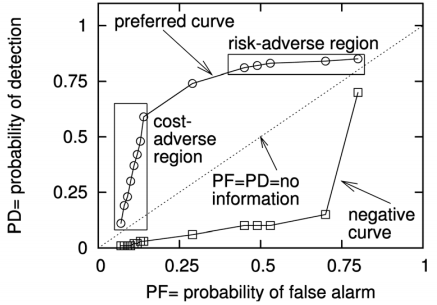
\includegraphics[width=2.0in]{roc.png}
\end{center}
\vspace{-0.2cm}
\caption{Trade-offs false alarm vs
recall (probability of detection).  }\label{fig:trade}
 \end{wrapfigure}
There are many more ways to evaluate defect predictors besides the four listed above.
Previously we have catalogued dozens of them (see Table 23.2 of~\cite{menzies2014sharing}) and even several novel ones were proposed
(balance, G-measure~\cite{menzies2007data}).  
No evaluation criteria is ``best'' since different  criteria are appropriate in different business contexts. For example, as shown
in 
Figure~\ref{fig:trade},
when dealing
with safety-critical applications, management may be
``risk adverse'' and hence many elect
 to {\em maximize recall}, regardless of the time wasted exploring  false alarm.
 Similarly, 
when rushing some non-safety critical application to market, management may be ``cost adverse''
and elect to {\em minimize false alarm} since this avoids distractions to the developers. 

In summary, there are  numerous evaluation criteria and  numerous more business contexts
where different criteria might be preferred by different local business users. In response to
the cornucopia of evaluation criteria, we make the following recommendations: a) do evaluate learners on more than one criteria, b) do not evaluate learners on  all criteria (there are too many), and instead, apply the criteria widely seen in the literature. Applying this advice, this paper  evaluates the defect predictors using the four criteria
mentioned above (since these are widely reported in the literature~\cite{ghotra2015revisiting,fu2016tuning})) but not other 
 criteria  that  have yet to gain a wide acceptance 
 (i.e., balance and G-measure).
 
% \begin{wrapfigure}{r}{1.8in}
%   \centering
%   \captionsetup{justification=centering}
%   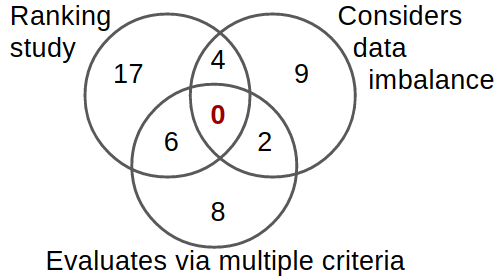
\includegraphics[width=1.8in]{venn.png}
%   \caption{Summary of  Table~\ref{tbl:survey2}.}
% \label{fig:s2}
% \end{wrapfigure}


\subsection{Defect Prediction and Class Imbalance}
\label{sect:imbalance}
  Class imbalance  is concerned with the situation in where some classes of data are
highly under-represented compared to other classes~\cite{he2009learning}.
By convention,
the under-represented class is called the {\em minority} class,
and correspondingly the class which is over-represented is called the
{\em majority} class. In this paper, we say that class imbalance is {\em worse}
when the ratio of minority class to majority {\em increases}, that is,
{\em class-imbalance of 5:95} is worse than {\em 20:80}. Menzies et al.~\cite{menzies2007problems} reported SE data sets often contain class imbalance. In their examples, they showed static code defect prediction data sets with
class imbalances of 1:7; 1:9; 1:10; 1:13; 1:16; 1:249. 


 \begin{table}[!b]
\centering
\footnotesize
\vspace{-0.4cm}
\caption{22 highly cited Software Defect prediction studies.}
\vspace{-0.2cm}
\label{tbl:survey2}
    \begin{tabular}{c|c|c|c|c|c}
        \begin{tabular}[c]{@{}c@{}}\textbf{Ref}\end{tabular} & \textbf{Year} & \textbf{Citations} & \begin{tabular}[c]{@{}c@{}}\textbf{Ranked} \\\textbf{Classifiers?} \end{tabular} &\begin{tabular}[c]{@{}c@{}} \textbf{Evaluated} \\\textbf{using} \\\textbf{multiple} \\\textbf{criteria?}\end{tabular}&\begin{tabular}[c]{@{}c@{}} \textbf{Considered}\\\textbf{Data}\\\textbf{Imbalance?} \end{tabular}\\ \hline
        \cite{menzies2007data} & 2007 & 855 & \cmark & 2 & \xmark \\
        \cite{lessmann2008benchmarking} & 2008 & 607 & \cmark & 1 & \xmark \\ 
        %\cite{hall2012systematic} & 2012 & 413 & \cmark & 3 & \xmark \\
        \cite{elish2008predicting} & 2008 & 298 & \cmark & 2 & \xmark\\  
        \cite{menzies2010defect} & 2010 & 178 & \cmark & 3 & \xmark \\  
        \cite{gondra2008applying} & 2008 & 159 & \cmark & 1 & \xmark\\     
        \cite{kim2011dealing} & 2011 & 153 &\cmark & 2 & \xmark \\ 
        \cite{radjenovic2013software} & 2013 & 150 & \cmark & 1 & \xmark \\   
        \cite{jiang2008techniques} & 2008 & 133 & \cmark & 1 & \xmark \\    
        \cite{wang2013using} & 2013 & 115 & \cmark & 1 & \cmark \\  
        \cite{mende2009revisiting} & 2009 & 92 & \cmark & 1 & \xmark \\          
        \cite{li2012sample} & 2012 & 79 & \cmark & 2 & \xmark  \\ 
        \cite{kamei2007effects} & 2007 & 73 & \xmark & 2 & \cmark\\  
        \cite{pelayo2007applying} & 2007 & 66 & \xmark & 1 & \cmark \\  
        \cite{jiang2009variance} & 2009 & 62 & \cmark & 3 & \xmark  \\ 
        \cite{khoshgoftaar2010attribute} & 2010 & 60 & \cmark & 1 & \cmark  \\  
        \cite{ghotra2015revisiting} & 2015 & 53 & \cmark & 1 & \xmark  \\  
        \cite{jiang2008can} & 2008 & 41 & \cmark & 1 & \xmark  \\  
         \cite{tantithamthavorn2016automated} & 2016 & 31 & \cmark & 1 & \xmark  \\ 
        \cite{tan2015online} & 2015 & 27 & \xmark & 2 & \cmark \\  
        \cite{pelayo2012evaluating} & 2012 & 23 & \xmark & 1 & \cmark \\  
        \cite{fu2016tuning} & 2016 & 15 & \cmark & 1 & \xmark  \\  
        \cite{bennin2017mahakil} & 2017 & 0 & \cmark & 3 & \cmark \\
\end{tabular}
\vspace{-0.3cm}
\end{table}

 \begin{table*}[!t]
 \caption{Classifiers used in this study.
 Rankings
 from Ghotra et al.~\cite{ghotra2015revisiting}.}
 \vspace{-0.2cm}
 \label{tbl:learners}
 \footnotesize
 \begin{tabular}{l|l|p{4.5in}}
{\bf RANK} & {\bf LEARNER} & {\bf NOTES}\\\hline
 1 ``best'' & RF= random forest & 
 Random forest of entropy-based decision trees.\\\cline{2-3}
 &  LR=Logistic regression &
 A generalized linear regression
model.\\\hline
 2 & KNN= K-means &  Classify a new instance by finding ``k'' examples of similar instances.
 Ghortra et al. suggested
 $K=8$.\\\cline{2-3}
 & NB= Naive Bayes &  Classify a new instance by (a)~collecting mean and standard deviations of attributes in old instances of  different classes; (b)~return the class whose attributes are statistically most similar to the new instance.\\\hline
 3 & DT= decision trees & Recursively
 divide data by selecting attribute splits
 that reduce the entropy of the class distribution.\\\hline

 4 ``worst'' & SVM= support vector machines &
 Map the raw data into a higher-dimensional space where it is easier to distinguish the examples.
 \\\hline
 \end{tabular}
 \vspace{-0.2cm}
 \end{table*}
 
 
The problem of class imbalance is sometimes discussed in the software analytics community.
Hall et al.~\cite{hall2012systematic} found that models based on C4.5 under-perform if they have imbalanced data while Naive Bayes and Logistic regression perform relatively better. 
Their general recommendation is to not use
imbalanced data.  
Some researchers offer preliminary explorations into methods that might mitigate for class imbalance.
Wang et al.~\cite{wang2013using} and Yu et al.~\cite{yu2017performance} validated the Hall et al. results and concluded that the
performance of C4.5 is unstable on imbalanced data sets while  Random Forest and Naive Bayes are 
more stable. 
Yan et al.~\cite{yan2010software} performed fuzzy logic and rules to overcome the imbalance problem, but they only
explored one kind of learner (Support Vector Machines).
Pelayo et al.~\cite{pelayo2007applying} studied the effects of the percentage of oversampling and undersampling done. They found out that different percentage of each helps improve the accuracies of decision tree learner for defect prediction using CK metrics. Menzies et al.~\cite{menzies2008implications} undersampled the non-defect class to balance training
data and reported how little information was required to learn a defect predictor. They found that throwing away data does not degrade the performance of Naive Bayes and C4.5 decision trees. Other papers~\cite{pelayo2007applying, pelayo2012evaluating, riquelme2008finding} have shown the usefulness of resampling based on different learners.

We note that  
many researchers in this area  (Wang, Yu et al., Gray et al.~\cite{gray2009using,yu2017performance,wang2013using}) refer to the {\sma} method explored in this paper,  but only in the context of future work.
 One rare exception to this general pattern is the recent TSE'17 paper by   Bennin et al.\cite{bennin2017mahakil}, which we explored as part of
RQ4.

% who compared many learners, with different class imbalance techniques evaluated against recall and false alarm. He selected the similar datasets which we have studied in this paper. He showed that among all the mentioned class imbalance techniques, their method and {\sma} outperform them in both the evaluation measures. Their method and {\sma} did perform same in terms of recall but their method faired on false alarm. But in this sample, no researcher has  applied auto-tuning to learn best {\sma} control parameters. We believe it to be an important factor and that is why we have provided the comparison between {\smb} and Bennin et al. method.}
 



 
 \subsection{Ranking Studies}
\label{sect:rank}

A constant problem in defect prediction is what  classifier should be applied to  build  the  defect  predictors?
To address this problem, many researchers run {\em ranking studies} where  performance scores 
are collected from  many classifiers  executed on  many software defect data sets~\cite{lessmann2008benchmarking,hall2012systematic,elish2008predicting,menzies2010defect,gondra2008applying,radjenovic2013software,jiang2008techniques,wang2013using,mende2009revisiting,li2012sample,khoshgoftaar2010attribute,jiang2009variance,ghotra2015revisiting,jiang2008can,tantithamthavorn2016automated,fu2016tuning}.
This section assesses those ranking studies. We will say a ranking study is ``good'' if it compares multiple learners using multiple data sets and multiple evaluation criteria
while at the same time doing something to address the data imbalance problem.


 \begin{wrapfigure}{r}{1.8in}
  \centering
  \captionsetup{justification=centering}
  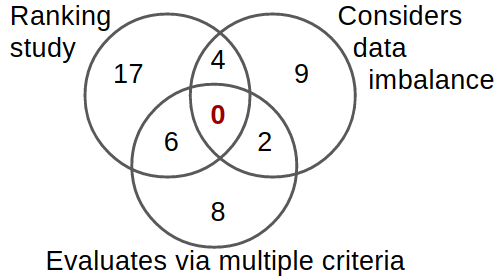
\includegraphics[width=1.8in]{venn.png}
  \caption{Summary of  Table~\ref{tbl:survey2}.}
\label{fig:s2}
\vspace{-0.4cm}
\end{wrapfigure}
In July 2017,  we searched
scholar.google.com for the conjunction of ``software'' and ``defect prediction'' and ``oo'' and ``ck'' published in the last decade. This returned 231 results.
We only selected oo and ck keywords since ck metrics are more popular and better than process metrics for software defect prediction~\cite{radjenovic2013software}.
From that list, we selected ``highly-cited'' papers, which we defined as having more than 10 citations per year. This reduced our population of papers down to 107.
After reading the titles and abstracts of those papers, and skimming the contents of the potentially interesting papers, we found 22 papers of Table~\ref{tbl:survey2} that either performed ranking studies
(as defined above) or studied the effects of class imbalance on defect prediction. In the column ``evaluated using
multiple criteria'',
papers scored more than ``1'' if they used multiple performance scores  of the kind listed at the end of \tion{performance}. 


We find that, in those 22 papers from Table~\ref{tbl:survey2},
numerous classifiers have used AUC as the measure to evaluate the software defect
predictor studies. We also found that majority of papers (from third column of Table~\ref{tbl:survey2}, 6/7=85\%) in SE community has used SMOTE to fix the data imbalance~\cite{wang2013using,kamei2007effects,pelayo2007applying,tan2015online,pelayo2012evaluating,bennin2017mahakil}. This also made us to propose {\smb}. As
 noted in~\cite{lessmann2008benchmarking, ghotra2015revisiting},  no single classification technique always dominates.  
That said, Table~IX of a recent study by Ghotra et al.~\cite{ghotra2015revisiting} ranks
 numerous classifiers  using data similar
 to what we use here (i.e., OO JAVA systems described using CK metrics).
  Using their work, we can
select
 a range of classifiers  for this study
 ranking from ``best''
 to ``worst': see Table~\ref{tbl:learners}.
 


%  \begin{figure}[!htbp]
% \begin{center}
% 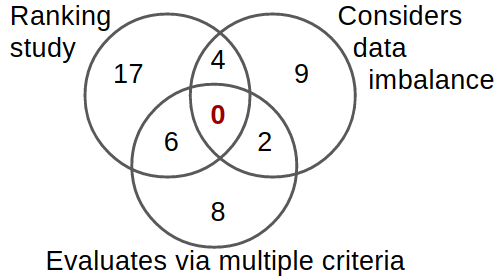
\includegraphics[width=2.5in]{venn.png}
% \end{center}
% \caption{Summary of papers from Table~\ref{tbl:survey2}.} 
% \label{fig:s2}
% \end{figure}
 
%\renewcommand\arraystretch{1.2}

% Accordingly, this paper is a ranking study that (a)~uses   multiple performance criteria to assess its classifiers; while (b)~fixing regions of the training
%  data with a weak signal  via synthetic data generation (using {\smb}, which is a self-tuning variant of {\sma}~\cite{chawla2002smote}). {\sma} is controlled by parameters which are normally set via ``expert judgement'' (a.k.a. guessing).
%  {\smb} uses a search-based SE technique called DE {\em differential evolution}~\cite{storn1997differential}) to automatically learn the best parameters for each data set. For more on {\smb}, see the next section.

% There are many studies done to find the best defect prediction performing model. Before 2007, it can be observed that almost every defect prediction study worked with 1 or 2 classification techniques evaluate on 1 or 2 measures. And almost none of the studies consider the effects of data imbalance. From Table~\ref{tbl:survey2} there has been ranking studies to find the best performing classifiers in about 16 out of 21 studies. Out of these 16, only 3 studied the effects of imbalance and among these 3 none studied for multiple evaluation goals.
% We highly agree to this given so many variations available in the data band there are so many classification techniques available like 

The key observation to be made from  this 
survey is that, as shown in Figure~\ref{fig:s2}, the overwhelming majority of
prior papers in our sample {\em do not satisfy}  our definition of a ``good'' project
(the sole exception is the  recent   Bennin et al.~\cite{bennin2017mahakil} which we explore in RQ4).
Accordingly, the rest of this
paper defines and executes a ``good'' ranking  study, with the added additional
unique feature of   an auto-tuning version of {\sma}.

\subsection{Handling Data Imbalance with SMOTE}
\label{sect:smote}

{\sma} handles class imbalance by changing the frequency of different classes of the training
data~\cite{chawla2002smote}. 
The algorithm's name is short for ``synthetic minority over-sampling technique''.
When applied to data, {\sma} sub-samples the majority class (i.e., deletes some examples)
while super-sampling the minority class
until
all classes have the same frequency.  In the case of software defect data,
the minority class is usually the  defective class.

Figure~\ref{fig:pseudocode} shows how {\sma} works. During super-sampling,
a member of the minority class finds $k$ nearest neighbors. It builds a fake member
of the minority class at some point in-between itself and one of its nearest
neighbors.  During that process, some distance function is required which is the {\em minkowski\_distance} function. 

{\sma}'s control parameters are (a) $k$ that selects how many neighbors to use  (defaults to $k=5$), (b) $m$ is how many examples of each class to generated (defaults to $m=50\%$ of the total training samples), and (3) $r$ which selects  the distance function (default is $r=2$,
i.e., use    
  Euclidean distance).

% Different data preprocessing has been proved
% to improve the performance of defect prediction models by
% Menzies et al.~\cite{menzies2007data}. Jiang et al.~\cite{jiang2008can} evaluate the impact of
% log transformation and discretization on the performance
% of defect prediction models, and report different modeling
% techniques ``prefer'' different transformation techniques. For
% instance, Naive Bayes achieves better performance on discretized
% data, while logistic regression achieves better performance
% for both. Peters et al.~\cite{peters2013better} propose different filters; and Li et al.~\cite{li2012sample} propose
% to use sampling. Nam et al.~\cite{nam2013transfer} transformed both
% training and testing data to the same latent feature space,
% and build models on the latent feature space. 
% %Too many variables in the datacan result in the ``curse of dimensionality''~\cite{friedman1997bias}.
% Feature Selection is a common method that can
% reduce features and sampling can balance the diversity of
% class instance numbers~\cite{yin2015empirical}, in turn improving the performance of defect prediction. In this paper we only tackle the class imbalance problem.


In the software analytics literature, there are contradictory findings on
the value of applying {\sma} for software defect prediction.
Van et al.~\cite{van2007experimental}, Pears et al.~\cite{pears2014synthetic} and Tan et al.~\cite{tan2015online} found {\sma} to be advantageous, while others, such as Pelayo et al.~\cite{pelayo2007applying} did not. 

 \begin{wrapfigure}{r}{2in}\small
\begin{lstlisting}[mathescape,linewidth=2in,frame=n,numbers=none]
  def SMOTE(k=2, m=50%, r=2):  # defaults
    while Majority > m do
      delete any majority item
    while Minority < m do
      add something_like(any minority item)
      
  def something_like(X0): 
    relevant = emptySet
    k1 = 0
    while(k1++ < 20 and size(found) < k)  {
       all = k1 nearest neighbors
       relevant += items in "all" of X0 class}
    Z = any of found
    Y = interpolate (X0, Z)
    return Y
    
  def minkowski_distance(a,b,r): 
    return $( \Sigma_i\ abs(a_i - b_i)^r)^{1/r}$
\end{lstlisting} 
\vspace{-0.2cm}
\caption{Pseudocode of SMOTE}
\label{fig:pseudocode} 
\vspace{-0.3cm}
\end{wrapfigure}

Further, some researchers report that some learners respond better than others to {\sma}. Kamei et al.~\cite{kamei2007effects} evaluated the effects of {\sma} applied to  four fault-proneness models
(linear discriminant analysis, logistic regression, neural network, and decision tree) by
using two module sets of industry legacy software. They reported that {\sma} improved the prediction performance of the linear and logistic models, but not neural network and decision tree models. Similar results, that the value of {\sma} was dependent on the learner,
was also reported by Van et al.~\cite{van2007experimental}.

Recently in TSE'17, Bennin et al.~\cite{bennin2017mahakil}  proposed a new method based on the chromosomal theory of inheritance. 
Their MAHAKIL algorithm interprets two distinct sub-classes as parents and generates a new synthetic instance that inherits different traits from each parent and contributes to the diversity within the data distribution.
They report that MAHAKIL usually performs as well as  {\sma}, but
does much better than all   other class balancing techniques in terms of recall.
Not that, that work did not  consider the impact of parameter tuning of a preprocessor so in our RQ4 we will compare {\smb} to MAHAKIL.

\subsection{SMOTUNED = auto-tuning {\sma}}
\label{sect:smotuned}

One possible explanation for the variability in the {\sma} results is that the
default parameters of this algorithm are not suited to all data sets. To test this,
we designed {\smb}, which is an auto-tuning version of {\sma}. {\smb}
uses different control parameters for different data sets.


 
{\smb} uses DE (differential evolution~\cite{storn1997differential}) to explore the parameter space of
Table~\ref{tb:tuned}.  DE is an
optimizer useful for functions that may not be smooth or linear.  Vesterstrom et al.~\cite{vesterstrom2004comparative} find   DE's optimizations to be  competitive with other optimizers like 
   particle swarm optimization or genetic algorithms.
   DEs have been used before for   parameter tuning~\cite{omran2005differential, chiha2012tuning,fu2016tuning,fu2017easy, agrawal2016wrong}) but this paper is  the first attempt to do
   DE-based class re-balancing.

\begin{figure}[!t]
\small 
\begin{lstlisting}[mathescape,linewidth=6.7cm,frame=none,numbers=right ]
  def DE( n=10, cf=0.3, f=0.7):  # default settings
    frontier = sets of guesses (n=10)
    best = frontier.1 # any value at all
    lives = 1
    while(lives$--$ > 0): 
      tmp = empty
      for i = 1 to $|$frontier$|$: # size of frontier
         old = frontier$_i$
         x,y,z = any three from frontier, picked at random
         new= copy(old)  
         for j = 1 to $|$new$|$: # for all attributes
           if rand() < cf    # at probability cf...
              new.j = $x.j + f*(z.j - y.j)$  # ...change item j
         # end for
         new  = new if better(new,old) else old
         tmp$_i$ = new 
         if better(new,best) then
            best = new
            lives++ # enable one more generation
         end                  
      # end for
     frontier = tmp
    # end while
    return best
\end{lstlisting} 
\caption{SMOTUNED uses DE (differential evolution).}
\label{fig:pseudo_DE} 
\vspace{-0.3cm}
\end{figure}


In Figure~\ref{fig:pseudo_DE}, DE evolves a \textit{frontier} of
candidates from an initial population which is driven by a goal (like maximizing recall) evaluated using a fitness function (shown in line 17). In the case of {\smb},
each  candidate is a randomly selected value for {\sma}'s $k, m$ and $r$ parameters.
 To evolve the frontier, within each generation,
 DE compares each item to a {\em new} candidate generated
 by combining three other frontier items (and better {\em new} candidates replace
 older items). 
 To compare them, the {\em better} function (line 17) calls $SMOTE$ function (from Figure~\ref{fig:pseudocode}) using the proposed {\em new} parameter settings. This pre-processed training data is then fed into a classifier to find a particular measure (like recall).
 When our DE  terminates, it returns the best candidate ever seen in the entire run.
 
Table~\ref{tb:algo2} provides an overview of {\smb} when exploring SMOTE's
  parameter ranges,  shown  in  Table~\ref{tb:tuned}. To define
the parameters, we found the range of used settings for {\sma} and distance functions
in the   SE and machine learning  literature.  Aggarawal et al.~\cite{aggarwal2001surprising}
argue that with data being highly dimensional, $r$ should shrink to some fraction less than one
(hence the bound of $r=0.1$ in Table~\ref{tb:tuned}. 


\begin{table}[!t]
    \begin{center}
    \footnotesize
\caption{SMOTE parameters}
\label{tb:tuned}
 \begin{tabular}{p{0.5cm}|c@{~}|c@{~}|p{3.3cm}}
         \textbf{Para} &  \begin{tabular}[c]{@{}c@{}}\textbf{Defaults} \\ \textbf{used by} \\\textbf{{\sma}} \end{tabular}
          &  \begin{tabular}[c]{@{}c@{}}
          \textbf{Tuning Range} \\
           \textbf{(Explored by} \\ \textbf{( {\smb})} \end{tabular}&  \textbf{Description} \\
        \hline
        $k$ & 5 & [1,20] & Number of neighbors \\ 
        \hline
       $m$ & 50\% & {50, 100, 200, 400} & Number of synthetic examples to create. Expressed as a percent  of final training data. \\ 
        \hline
        $r$ & 2 & [0.1,5] & Power parameter for the Minkowski distance metric.\\
 
\end{tabular}
\end{center}
\end{table}

\begin{table}[!t]
\begin{center}
\footnotesize
\caption{SMOTUNED parameters}
\label{tb:algo2}
\begin{tabular}{|c@{~}|p{4.0cm}|}
        \hline 
        \textbf{Keywords} & \textbf{Description}\\
        \hline

        \begin{tabular}[c]{@{}c@{}}Differential weight $(f=0.7)$\end{tabular} & Mutation power\\
        \hline
        \begin{tabular}[c]{@{}c@{}}Crossover probability $(cf=0.3)$\end{tabular} & Survival of the candidate\\
        \hline
        \begin{tabular}[c]{@{}c@{}}Population Size $(n=10)$\end{tabular} &  Frontier size in a generation \\
        \hline
        \begin{tabular}[c]{@{}c@{}}Lives\end{tabular} & Number of generations\\
        \hline
        \begin{tabular}[c]{@{}c@{}}Fitness Function $(better)$\end{tabular} & Driving factor of DE\\
        \hline
        \begin{tabular}[c]{@{}c@{}}Rand() function\end{tabular} & Returns between 0 to 1 \\
        \hline
        \begin{tabular}[c]{@{}c@{}}Best (or Output)\end{tabular} & Optimal configuration for {\sma} \\
        \hline
\end{tabular}
\end{center}
\end{table}
 


\section{Experimental Design}
\label{sect:experiment}
 
This experiment  reports the effects on   defect prediction
after using MAHAKIL or {\smb} or {\sma}. 
 
 \begin{table}[!b]
\begin{center}
\small
\caption{Data set statistics. Data sets are sorted from low percentage of defective class to high defective class.
Data comes from the SEACRAFT repository: http://tiny.cc/seacraft}.
\vspace{-0.2cm}
\label{tb:dataset}

\begin{tabular}{r@{~}|r@{~}|r@{~}|r@{~}|r@{~}|r@{~}}
\footnotesize
        \begin{tabular}[c]{@{}c@{}}\textbf{Version}\end{tabular} & \begin{tabular}[c]{@{}c@{}} \textbf{Dat aset} \\ \textbf{Name}\end{tabular} & \textbf{Defect \%} & \textbf{Non-Defect \%} &\begin{tabular}[c]{@{}c@{}} \textbf{No. of} \\ \textbf{classes}\end{tabular}&\begin{tabular}[c]{@{}c@{}} \textbf{lines of} \\ \textbf{code} \end{tabular}\\ \hline
4.3 & jEdit & 2 & 98 & 492 & 202,363 \\ 
1.0 &   Camel & 4 & 96 & 339 & 33,721 \\  
6.0.3 &   Tomcat & 9 & 91 & 858 & 300,674\\ 
2.0 &   Ivy & 11 & 89 & 352 & 87,769 \\  
1.0 & Arcilook & 11.5 & 88.5 & 234 & 31,342\\ 
1.0 & Redaktor & 15 & 85 & 176 & 59,280 \\ 
1.7 & Apache Ant & 22 & 78 & 745 & 208,653 \\  
1.2 &   Synapse & 33.5 & 66.5 & 256 & 53,500 \\ 
1.6.1 &   Velocity & 34 & 66 & 229 & 57,012 \\\hline
  \multicolumn{4}{r|}{ total:} &    3,681&	1,034,314\\ 

\end{tabular}
\end{center} 
\end{table}

\newcommand\fnote[1]{\captionsetup{font=small}\caption*{#1}}

\begin{figure*}[!b]
    \centering
    \begin{minipage}{.33\textwidth}
    \centering
    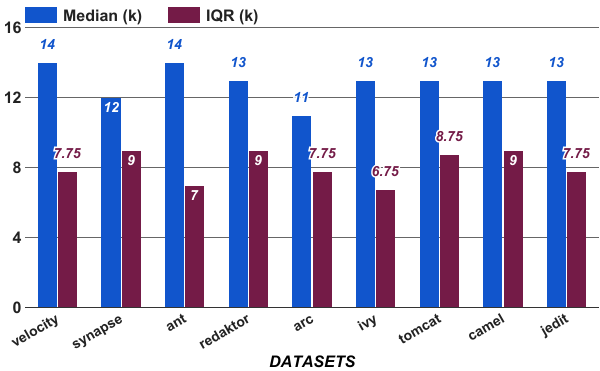
\includegraphics[width=.95\linewidth]{./fig/k.png}
        {\bf Figure~\ref{fig:para}a:} Tuned values for $k$\\ (default:  $k=5$).
    \end{minipage}~~%
    \begin{minipage}{.33\textwidth}
    \centering
        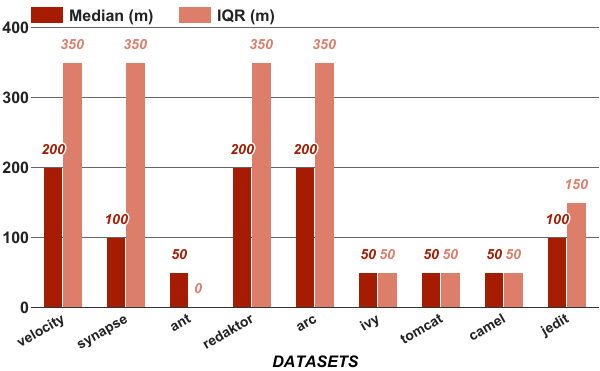
\includegraphics[width=.95\linewidth]{./fig/m.png}
        {\bf Figure~\ref{fig:para}b:} Tuned values for $m$\\ (default: $m=50\%$).
    \end{minipage}~~%
    \begin{minipage}{.33\textwidth}
    \centering
        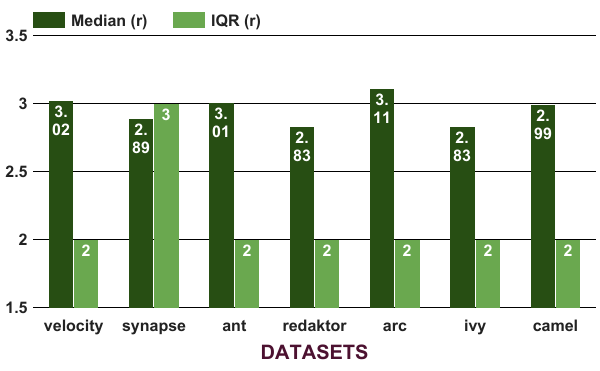
\includegraphics[width=.95\linewidth]{./fig/r.png}
        {\bf Figure~\ref{fig:para}c:} Tuned values for $r$\\ (default:  $r=2$).
    \end{minipage}
    \vspace{-0.2cm}
    \caption{Data sets vs Parameter Variation when optimized for recall and results reported on recall.
    ``Median'' denotes 50th percentile values seen in the 5*5 cross-validations and ``IQR'' shows the intra-quartile
    range, i.e., (75-25)th percentiles.}
    \label{fig:para}
\end{figure*}

 

Using some data $D_i \in D$, performance measure $M_i \in M$, and classifier $C_i \in C$,
this experiment conducts the 5*5 cross-validation study, defined below.
Our data sets  $D$ are shown in  Table~\ref{tb:dataset}. These are all open source
JAVA OO systems described in terms of the CK metrics described. 
Since, we are comparing these results for imbalanced class, only imbalanced class data sets are selected. 



Our performance measures $M$ were introduced in \tion{performance}
which includes   AUC, precision, recall, and the  false alarm. 
Our classifiers
 $C$  come from a  recent ICSE paper~\cite{ghotra2015revisiting}
and were listed in  Table~\ref{tbl:learners}.
For  implementations 
of these learners,
we used  the open source tool
Scikit-Learn~\cite{pedregosa2011scikit}.
Our  cross-validation study~\cite{refaeilzadeh2009cross} was defined as follows:
\be
\item We randomized the order of the data set $D_i$ set five times. This reduces the probability
that some random ordering of examples in the data will conflate our results.
\item Each time, we divided the data $D_i$ into five bins;
\item For each bin (the test), we trained on four bins (the rest) and then tested
on the test bin as follows.
\be
\item
Important point: {\em we only {\sma} the training data,  leaving
the  testing data unchanged}.
\item
The  training set is pre-filtered using either No-SMOTE (i.e., do nothing) or  {\sma} or {\smb}.  
\item
When using {\smb}, we further divide those four bins of training data. 3 bins are used for training the model, and 1 bin is used for validation in DE. DE is  run to  improve
the performance measure $M_i$ seen when the classifier $C_i$ was applied to the training data.
Important note: {\em when tuning {\sma}, this rig \underline{{\em never}} uses test data}.
\item
After pre-filtering, a classifier $C_i$  learns a predictor.
\item
The model is applied to the test data to collect performance measure $M_i$. 
\item 
We print the {\em performance delta} between this $M_i$ and another  $M_i$
generated from applying $C_i$ to the raw data $D_i$ (i.e., compared to learning
without any filtering).
\ee
\ee



\begin{figure*}[!t]
\begin{minipage}{.5\linewidth}
\centering
 
        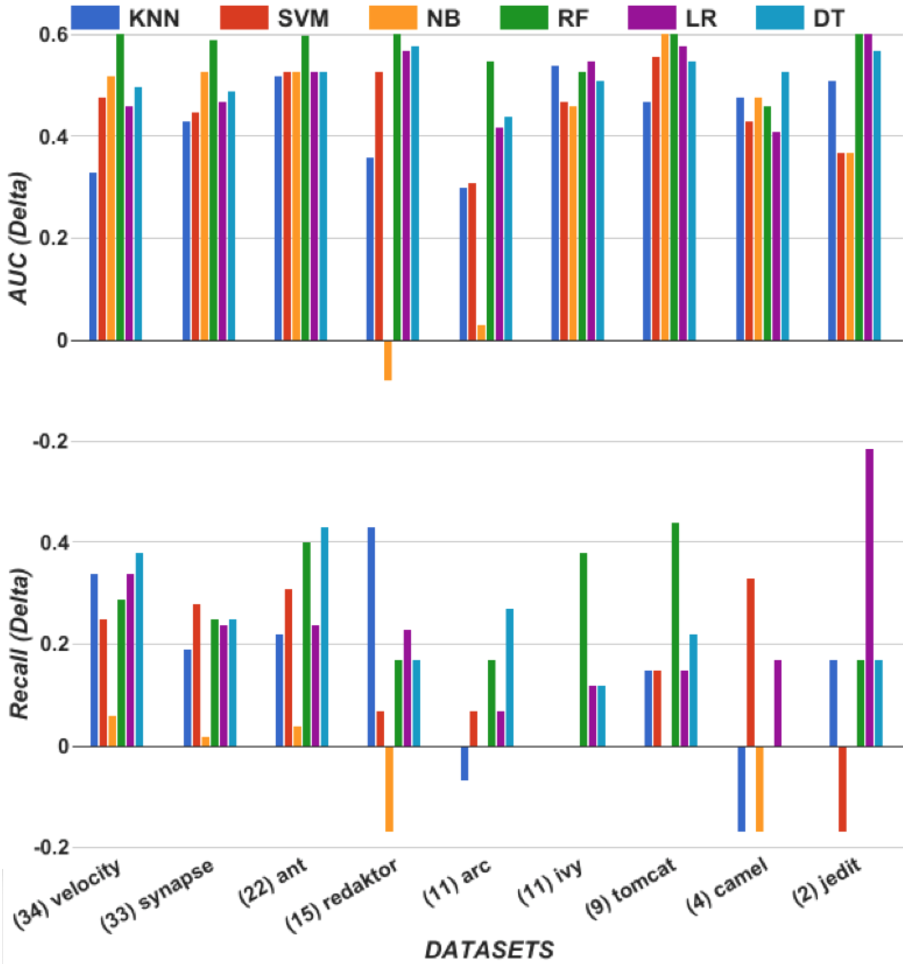
\includegraphics[width=0.75\linewidth,keepaspectratio,trim=0cm 1cm 0cm 2cm]{./fig/AUC_recall_tuned.png}
    \end{minipage}%
\begin{minipage}{.5\linewidth}
        \centering
        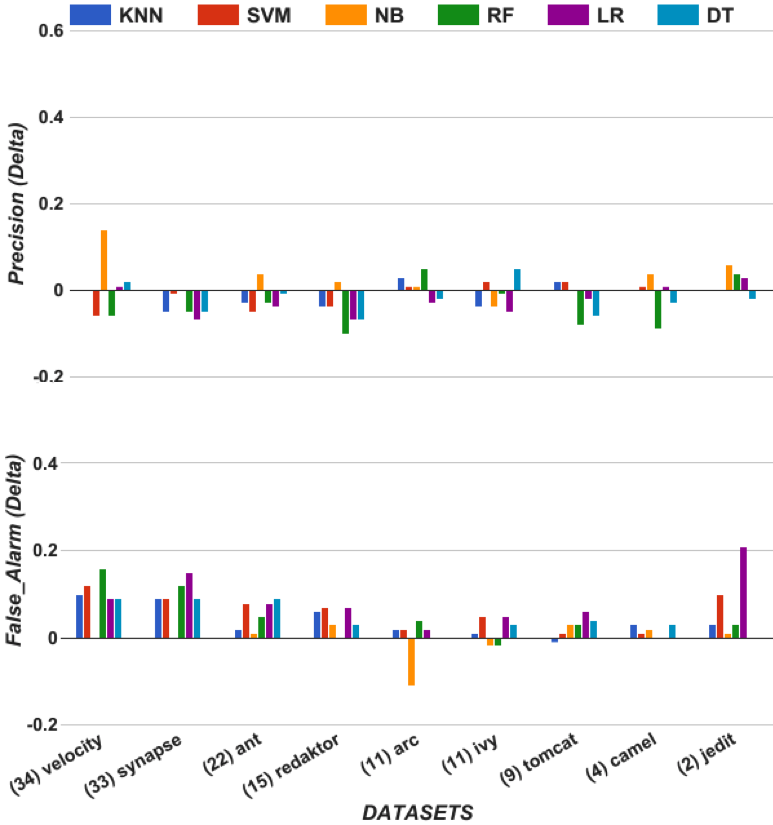
\includegraphics[width=0.75\linewidth,keepaspectratio,trim=0cm 1cm 0cm 2cm]{./fig/prec_pf_tuned.png}
    \end{minipage}%
    
    \caption{{\smb} improvements over {\sma}. \underline{Within}-Measure
    assessment (i.e., for each of these charts,
    optimize for performance measure $M_i$, then test for
    performance measure $M_i$). For most charts,
    {\em larger} values are {\em better}, but for false alarm,
    {\em smaller} values are {\em better}. Note that the corresponding percentage of minority class (in this case, defective class) is written beside each data set.}
    \label{fig:tuned}
\end{figure*}


 
   
   
Note that the above rig tunes {\sma}, but not the control parameters of the classifiers.
We do this since, in this paper,  we aim to document the   benefits of tuning {\sma} since as shown below, they are very large indeed. Also, it would be very useful if we can show that a single algorithm ({\smb})  improves the performance of defect prediction. This would allow
subsequent work to focus on the task of optimizing  {\smb} (which would be a far easier
task than optimizing the tuning of a wide-range of classifiers). 
 

\subsection{Within- vs Cross-Measure Assessment}
\label{sect:wcm}

We call the above rig as the {\em within-measure assessment rig} since it is  biased in its evaluation measures. Specifically,  in this rig,
when {\smb} is optimized for (e.g.,) AUC, we do not explore the effects on (e.g.,) the false alarm. This is less than ideal
since it is known that our performance measures are inter-connected via the Zhang's equation~\cite{zhang2007comments}. Hence, increasing (e.g.,) recall might potentially have the adverse
effect of  driving up (e.g) the false alarm rate. 
To avoid this problem, we also apply the following {\em cross-measure assessment rig}.
At the conclusion of the {\em within-measure assessment rig}, we will observe  that the AUC performance measure will show the largest improvements. Using that best performer, we will re-apply steps 1,2,3 abcdef (listed above) but this time:
\bi
\item In step 3c, we will tell {\smb} to optimize for AUC;
\item In step 3e, 3f we will collect the performance delta on AUC as well as precision, recall,
and false alarm.
\ei
In this approach, steps 3e and 3f collect the information required   to check if succeeding according to one performance criteria results in damage to another. We would also want to make sure that our model is not over-fitted based on one evaluation measure. And since {\smb} is a time expensive task, we do not want to tune for each measure which will quadruple the time. The results of within- vs cross-measure assessment is shown in Section \ref{sect:results}.


\subsection{Statistical Analysis}
\label{sec:scott-knott}

When comparing the results of {\smb} to other
treatments, we use a statistical
significance test and an effect size test.
Significance test are useful for detecting if two populations
differ merely by random noise. 
Also, effect sizes are useful for checking that two populations differ by more than just a trivial amount.

For the significance test,  we use the 
     Scott-Knott procedure  recommended at TSE'13~\cite{mittas2013ranking} and ICSE'15~\cite{ghotra2015revisiting}. This
     technique recursively bi-clusters a sorted
    set of numbers. If any two clusters are statistically indistinguishable, Scott-Knott
    reports them both as one group.
    Scott-Knott first looks for a break in the sequence that maximizes the expected
    values in the difference in the means before and after the break.
    More specifically,  it  splits $l$ values into sub-lists $m$ and $n$ in order to maximize the expected value of differences  in the observed performances before and after divisions. For e.g., lists $l,m$ and $n$ of size $ls,ms$ and $ns$ where $l=m\cup n$, Scott-Knott divides the sequence at the break that maximizes:
     \[E(\Delta)=ms/ls*abs(m.\mu - l.\mu)^2 + ns/ls*abs(n.\mu - l.\mu)^2\]
Scott-Knott then applies some statistical hypothesis test $H$ to check if $m$ and $n$ are significantly different. If so, Scott-Knott then recurses on each division.
    For this study, our hypothesis test $H$ was a conjunction of the A12 effect size test (endorsed by
    \cite{arcuri2011practical})  and non-parametric bootstrap sampling \cite{efron94}, i.e., our Scott-Knott divided the data if {\em both}
    bootstrapping and an effect size test agreed that the division was statistically significant (99\% confidence) and not a ``small'' effect ($A12 \ge 0.6$).
   

\begin{figure*}[!t]
\begin{minipage}{.49\linewidth}
\centering
        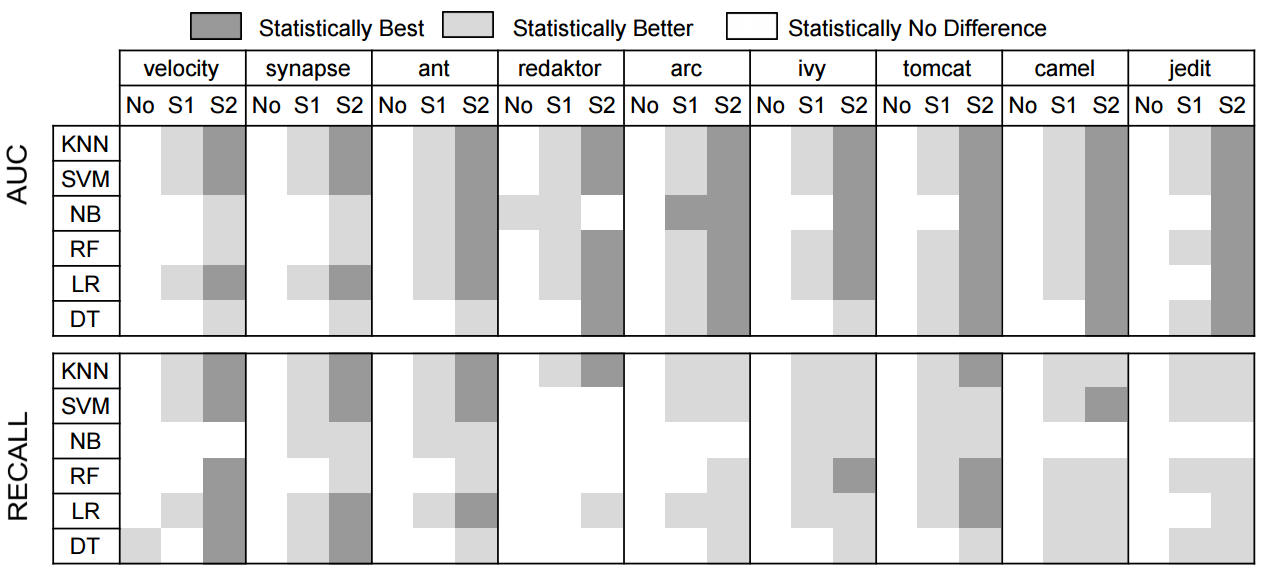
\includegraphics[width=\linewidth ]{./fig/AUC_recall.png}
            \end{minipage}%
\begin{minipage}{.49\linewidth}
        \centering
        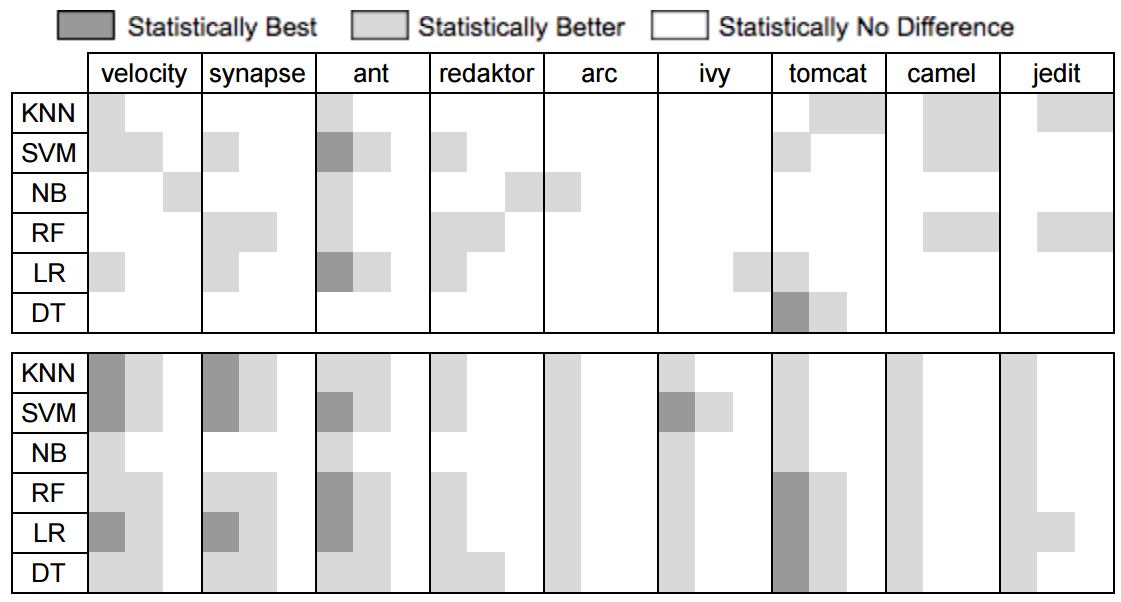
\includegraphics[width=\linewidth]{./fig/prec_pf.png}
    \end{minipage}%
    \caption{Scott Knott analysis of No-SMOTE, SMOTE and SMOTUNED. The column headers are denoted as No for No-SMOTE, S1 for SMOTE and S2 for SMOTUNED. $(\ast)$ Mark represents the best learner combined with its techniques.}
    \label{fig:stats}
\end{figure*}

\section{Results}
\label{sect:results}

{\bf RQ1: Are the default ``off-the-shelf'' parameters for SMOTE appropriate for all
 data sets?}
 
 As discussed above, the default parameters for
 {\sma}, $k,\ m$ and $r$ are $5,\ 50\%$ and $2$.
  Figure~\ref{fig:para} shows the range of parameters
 found by {\smb} across  nine data sets for the 25 repeats of our cross-validation procedure.
 All the results in this figure are {\em within-measure assessment} results, i.e.,
 here, we {\smb}  on a particular performance measure and then we only collect performance for that performance measure on the test set.
 
 
 In  Figure~\ref{fig:para}, the {\em median} is the 50th percentile
 value and {\em IQR} is the (75-25)th percentile
 (IQR is a non-parametric analogue of variance).
 As can be seen in Figure~\ref{fig:para}, most of the learned parameter are far from the default values:
 \bi
 \item 
 Median $k$ value was never less than 11,
 \item
 Median $m$ value differs according to each data set and quite far from the actual,
 \item
 The $r$ value used in the distance function was never 2. Rather, it was usually 3.
 \ei
 Hence,  our answer to {\bf RQ1} is ``no'': the use of off-the-shelf {\sma} should be deprecated. 
 
 Before moving on to {\bf RQ2}, we note that many of the settings in Figure~\ref{fig:para} are very similar; for example, median values of $k=13$ and $r=3$ seems to be a common
result.  Nevertheless, we do {\em not} recommend replacing
the defaults on regular {\sma} with the median values
of Figure~\ref{fig:para}. In that figure, many of the  IQR bars are
very large. Clearly, {\smb}'s decisions vary dramatically
depending on what data  is being processed.  Accordingly,
we strongly recommend that {\smb} be applied to each new data set.

\noindent
{\bf \\RQ2: Is there any benefit in tuning the default parameters of SMOTE for each new data set?}

Figure~\ref{fig:tuned} shows the performance delta of the {\em within-measure assessment rig}.
Please recall that when this rig applies {\smb}, it optimizes for performance measure, $M_i \in \{recall,\ precision,\ false$ $\ alarm,\ AUC\}$
after which it uses the {\em same} performance measure
$M_i$ when evaluating the test data. In Figure~\ref{fig:tuned}, each subfigure shows that DE is optimized for each $M\_i$ and results are reported against the same $M\_i$.
From the figure~\ref{fig:tuned}, it is observed that
{\smb} achieves large AUC (about 60\%) and recall (about 20\%) improvements
without
 damaging precision and  with only minimal changes
 to false alarm. A special note should be taken of the AUC improvements, that these are the largest improvements
 we have yet seen, for any prior treatment of defect prediction data.

Figure~\ref{fig:stats} offers a statistical analysis
of different results achieved
after applying our three data pre-filtering methods: 1) {\em \textbf{NO}} = do nothing, 2) {\em \textbf{S1}} = use default {\sma}, and 3) {\em \textbf{S2}} = use {\smb}.
For any learner, there are three such treatments and {\em darker} the cell, {\em better} the performance. 
In that figure, cells with the same color are
either not statistically significantly different or
are different only via a {\em small effect}
(as judged by the statistical methods described above).

As to what combination of pre-filter+learner works better for any data set, that is marked by a ``*''. Since we have three pre-filtering methods and six learners, there is one   ``*'' per 18 cells in Figure~\ref{fig:stats}.

In the  AUC and recall results,  the best ``*'' cell always appears in the S2={\smb} column, i.e.,  
 {\smb} is always
used by the best combination of pre-filter+learner .

As to precision  results,  at first glance, the  results in Figure~\ref{fig:stats} look bad for {\smb} since, less than half the times, 
the best ``*''  happens  in S2={\smb} column.
 But recall from Figure~\ref{fig:tuned} that the absolute size of the precision deltas is very small.  Hence, even though {\smb} ``losses'' in this statistical analysis, the pragmatic impact of that result  is  negligible.
 
As to the false alarm results from Figure~\ref{fig:stats}, as discussed above in \tion{performance}, the cost of increased recall is to also increase
the false alarm rate. For example, the greatest \textit{increase} in the recall was 0.58 seen in the {\em jEdit} results. This increase comes at a cost
of \textit{increasing} the false alarm rate by 0.20. Apart from this one large outlier, the overall pattern is that the recall improvements range from +0.18 to +0.42 (median to max)
and these come at the cost of much smaller false alarm \textit{increase} of 0.07 to 0.16 (median to max). 
 
In summary, the answer to {\bf RQ2} is that our  AUC and recall results strongly endorse the  use of {\smb}
while the precision and false alarm rates
show there is little harm in using {\smb}.

Before moving to the next research question, we note that these
 results offer an interesting insight on prior ranking studies.
%as ``better'' than another.
% Recall from Table~\ref{tbl:learners} that prior studies have offered an approximate ranking for different learners; specifically: $
% (\mathit{RF},\mathit{LR}) > (\mathit{KNN},\mathit{NB}) > (\mathit{DT}) > (\mathit{SVM})$
% If we count how often our learners perform
% best in the AUC and recall results of Figure~\ref{fig:stats} (i.e., how many times they were marked with ``*'') then, at first
% glance, it would seem that Figure~\ref{fig:stats} is recommending very nearly the same
% learners as ``best'' for defect prediction as   Table~\ref{tbl:learners}: $\begin{array}{c}
% (\mathit{RF}=7) > (\mathit{LR}=5) > (\mathit{KNN}=4) >\\
% (\mathit{SVM}=2) > (\mathit{NB}=0, \mathit{DT}=0)
% \end{array}$
% Here, we do not count  the precision and false alarm counts since, as discussed above, the size
% of that delta is so small (particularly when compared to the AUC+recall effects).
% \begin{figure}[!t]
% \centering
%         \begin{center}
%         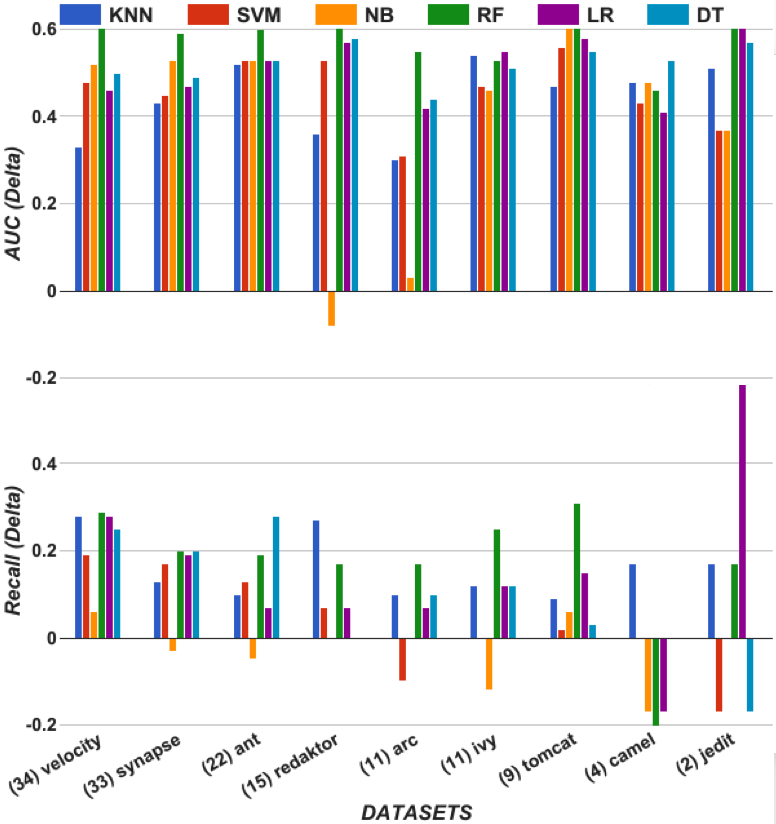
\includegraphics[width=0.8\linewidth,keepaspectratio]{./fig/AUC_auc1.png}
%         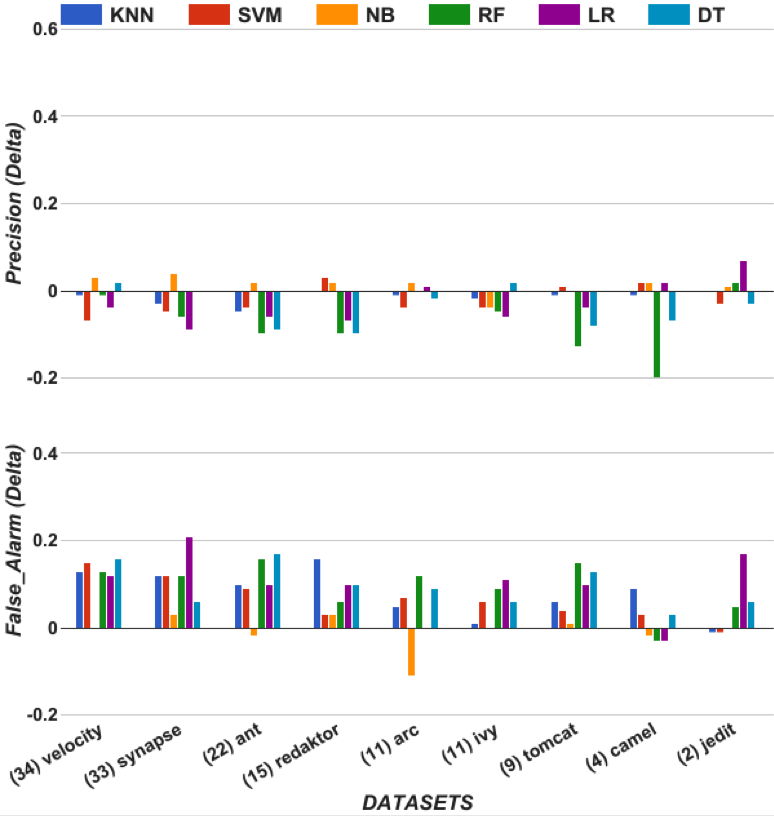
\includegraphics[width=0.8\linewidth,keepaspectratio]{./fig/AUC_prec.png}
%   \end{center}
%      \caption{ SMOTUNED improvement over SMOTE. 
%     \underline{{\bf Cross}}-Measure
%     assessment (i.e., for each of these charts,
%     optimize for \underline{{\bf AUC}}, then test for 
%     performance measure $M_i$).  Same format as
%     Figure~\ref{fig:tuned}.}
%     \label{fig:auc22}
% \end{figure}
Based on the Ghotra et al.
results of  Table~\ref{tbl:learners}, our expectation was that Random Forests (RF)
would yield the best results across this defect data. Figure~\ref{fig:stats} reports
that, as predicted by Ghotra et al., RF earns more ``stars'' than any other learner, i.e., it is seen to be ``best'' more often than anything else. That said,  
RF was only ``best'' 
in   11/36 of those results, i.e., even our ``best'' learner (RF) fails over half the time.

On the other hand, it is significant to note that
  {\smb} was  consistently  used  by  whatever  learner  was  found  to  be ``best'' (in recall and AUC). 
Hence, we conclude   prior ranking study results (that only assessed different learners) have missed a much more general effect; i.e.  
it an be more useful to reflect on data pre-processors that algorithm selection.
To say that another way, at least for defect prediction,
``better data'' might be better than ``better data miners''.

% As a last note about the {\bf RQ2} results, we note that they offer a new insight into
% the true value of methods of {\sma}.
% When we drew the plots of  Figure~\ref{fig:tuned}, we deliberately ordered
% the x-axis data sets according to their imbalance, 1) The data sets with the {\em highest} ratio of defects (Velocity and Synapse) are shown on the left-hand side of each plot in Figure~\ref{fig:tuned}, and 2) While the data sets with the {\em lowest} ratio of defects (jEdit and Camel) are shown on the right-hand side.

% Given that ordering of the x-axis, repairing class imbalance should improve the performance as we move from left to right hand side of the  Figure~\ref{fig:tuned} plots.
% But this is not the case (and effect size tests confirm that visual impression).
% Hence, we conjecture that the   real value of {\sma} (and {\smb}) is not fixing the class imbalance, rather, SMOTE's
% value might be in {\em amplifying} the data's signal in sparse regions of the data (by filling
% in those regions with synthetic examples extrapolated from the local region). 

\noindent
{\bf \\RQ3: In  terms  of  runtimes,  is  the  cost  of  running  SMOTUNED worth the performance improvement?}

Figure \ref{runtime} shows the mean runtimes
for running a 5*5 cross-validation study for six learners for each data set.
These runtimes were collected from one machine running CENTOS7, with 16 cores.
Note that they do not increase monotonically with the size of the data sets--  a result we can explain with respect to the internal
structure of the data.
Our version of {\sma} uses ball trees to optimize the nearest neighbor calculations. Hence, the runtime of that algorithm is dominated by the internal topology of the data sets rather than the number of classes.
Also, as shown in 
Figure~\ref{fig:pseudocode},
{\smb} explores the local space until it finds $k$ neighbors of the same class. This can take a variable amount of time to terminate.

 \begin{figure}[!htbp]
  \centering
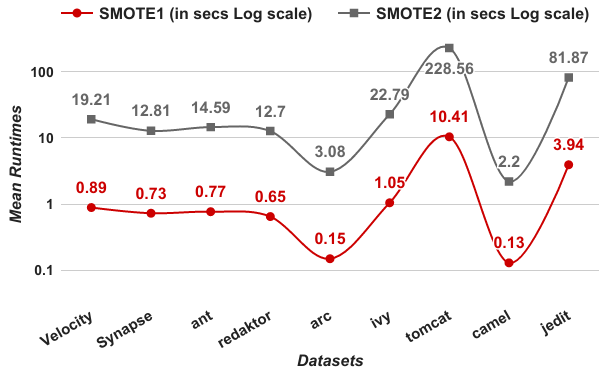
\includegraphics[width=3.0in,keepaspectratio]{./fig/runtimes.png}
  \caption{Data sets vs Runtimes. Note that the numbers
  shown here are the mean times seen across 25 repeats of a 5*5 cross-validation study.
  %running six learners through a 5*5 cross-validation. Hence, for mean
  %runtimes for one learner, {\em divide} these numbers by 6*5*5=150.
  }
  \label{runtime}
\end{figure}

\begin{figure*}[!t]
\begin{minipage}{.5\linewidth}
\centering
        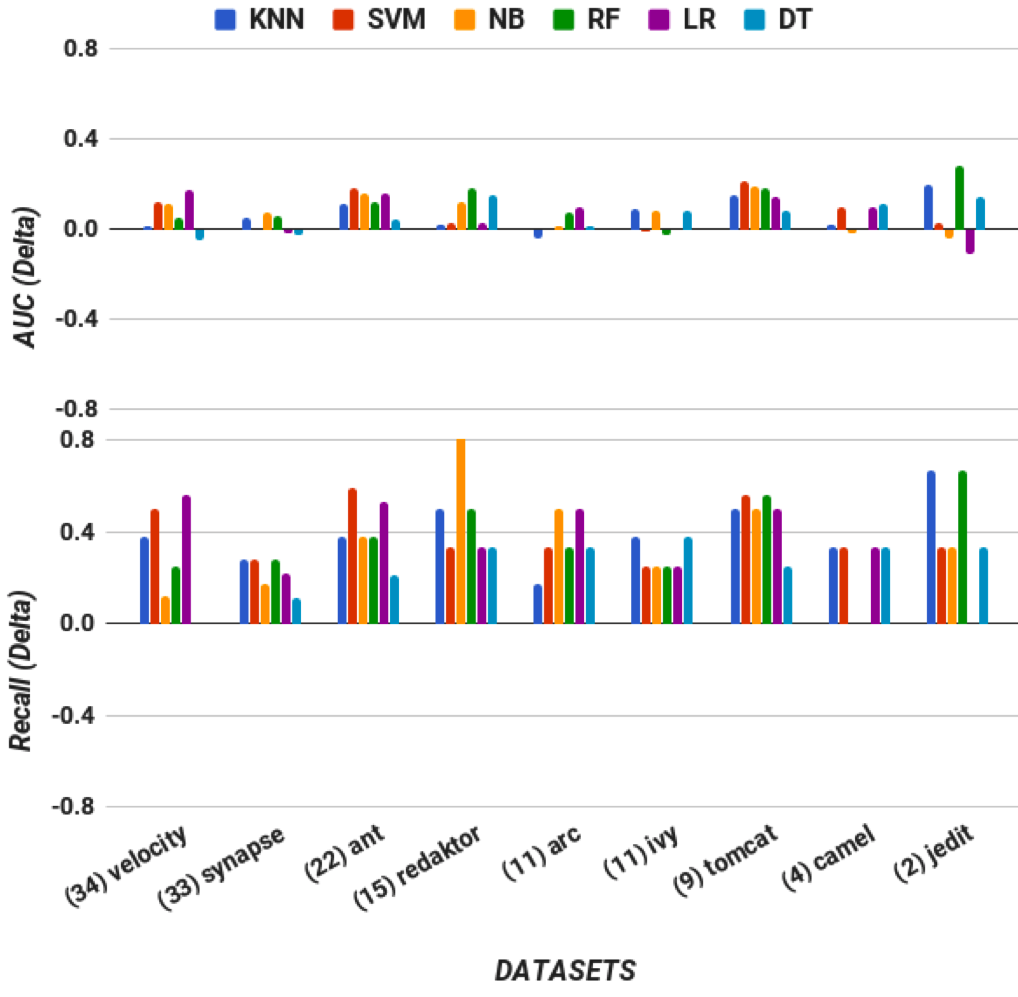
\includegraphics[width=0.75\linewidth,keepaspectratio,trim=1cm 1cm 1cm 1cm]{./fig/auc_recall_s2_maha.png}
    \end{minipage}%
\begin{minipage}{.5\linewidth}
        \centering
        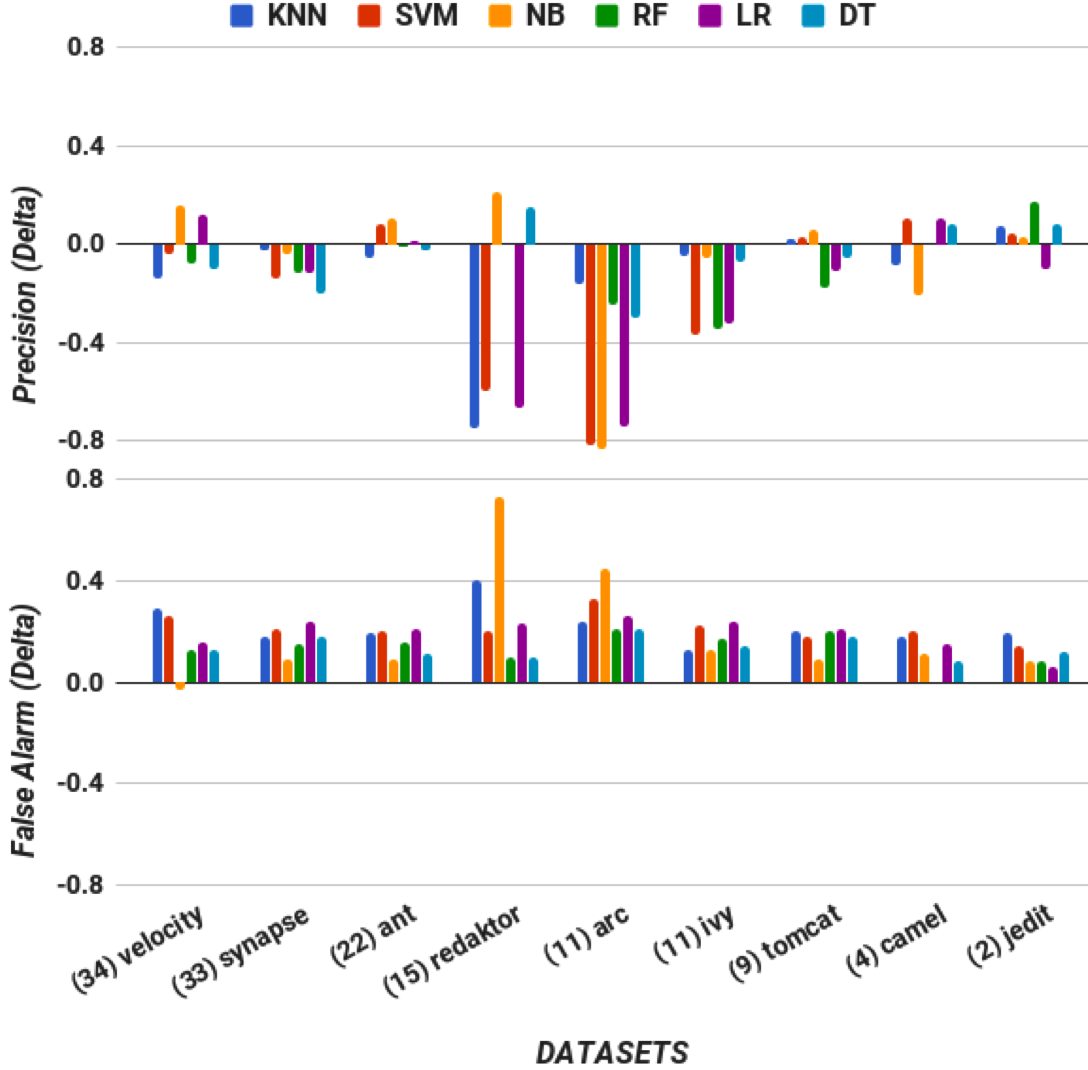
\includegraphics[width=0.75\linewidth,keepaspectratio,trim=1cm 1cm 1cm 1cm]{./fig/prec_pf_s2_maha.png}
    \end{minipage}%
    
    \caption{SMOTUNED improvements over MAHAKIL~\cite{bennin2017mahakil}. \underline{Within}-Measure
    assessment (i.e., for each of these charts,
    optimize for performance measure $M_i$, then test for
    performance measure $M_i$). Same format as  Figure~\ref{fig:tuned}.  }
    \label{fig:s2_mahakil}
\end{figure*}


As expected,  {\smb} is an order of magnitude slower than {\sma} since
it has to run {\sma} many times to assess different parameter settings.
That said, those runtimes are not excessively slow.
{\smb} usual terminates in under two minutes and never more than half an hour.
% Figure~\ref{runtime} by 5*5*6=150, we see that even for our slowest data sets (tomcat), one run
% of SMOTUNED terminated in 34284/150=228 seconds (on an average), which is less than four minutes.
Hence, in  our opinion, we answer {\bf RQ3} as ``yes'' since the   performance increment
seen in Figure~\ref{fig:tuned} is more than to compensate for the extra CPU required for {\smb}.

\noindent
{\bf \\RQ4: How does SMOTUNED performed against more recent class imbalance technique?}

All the above work is based on tuning the original 2002 {\sma} paper~\cite{chawla2002smote}. While that
version of {\sma} is widely used in the SE literature, 
it is prudent to compare {\smb} with more recent work.
Our reading
of the literature is that the MAHAKIL algorithm  of Bennin et al. in TSE 2017~\cite{bennin2017mahakil} represents the most recent work in  SE on handling  
class imbalance.  
At the time of writing of this paper (early August 2017), there was no reproduction package available for MAHAKIL so we wrote our own version
based on the description in that paper %(Reproduction Package blinded for review). 
(Available to download from https://github.com/ai-se/MAHAKIL\_imbalance).

Figure~\ref{fig:s2_mahakil} compares   results from MAHAKIL with those from {\smb}. These results
were generated using the same experimental methods as used for   Figure~\ref{fig:tuned} (those methods were described in  Section~\ref{sect:wcm}).
The following table repeats   the statistical analysis of Figure \ref{fig:stats} to report how often
  {\sma}, {\smb}, or MAHAKIL achieves best results across nine data sets.   Note that, in this following table, {\em larger} values are {\em better}:

{\small\[\begin{array}{*{20}{c|c|c|c|c}}
  & \multicolumn{4}{c}{\text{number of wins}}\\ 
    {\text{Treatments}} & {\text{AUC}} & {\text{Recall}} & {\text{Precision}}& {\text{False Alarm}}\\
    \hline
   {\text{MAHAKIL}} & 1/9 & 0/9 & \textbf{6/9} & \textbf{9/9}  \\
   {\text{SMOTE}}& 0/9 & 1/9 & 0/9 & 0/9 \\
   {\text{SMOTUNED}}& \textbf{8/9} & \textbf{8/9} & 3/9  & 0/9  \\
 \end{array} \]}

These statistical tests tell us that the differences seen in Figure~\ref{fig:s2_mahakil}  are large enough to be significant.  
\bi
\item
  Looking at Figure~\ref{fig:s2_mahakil}, the differences in precision
  are   so small
in most data sets (7/9) that the pragmatic impact of those differences   is negligible.
\item
As to AUC and recall,  we see that 
{\smb} generated   larger and better results than MAHAKIL (especially for recall).
\item
{\smb} generates slightly larger false alarms but, in 7/9 data sets,
the increase in the false alarm rate is usually very small.
\ei
According to its authors~\cite{bennin2017mahakil},
MAHAKIL was developed to reduce the false alarm rates on SMOTE and on that criteria it succeeds
 (as seen in  Figure~\ref{fig:s2_mahakil}, since {\smb} does lead to slightly higher false
alarm rates).   But, as discussed above in \ref{sect:performance}, the downside on minimizing false alarms is also minimizing our ability to 
find defects and, measured in terms of AUC and recall, {\smb} does best.
  Hence,  if this paper was a comparative assessment of  {\smb} vs MAHAKIL, we would conclude that
  by recommending {\smb}.

However, the goal of this paper is to defend the claim that ``better data'' could be better than ``better
data miners'', i.e., data pre-processing is more effective  than switching to another data miner.
In this regard,   there is something insightful to conclude if we combine the results of {\em both}
MAHAKIL and {\smb}.  
In the MAHAKIL experiments, the researchers spent some time parameter
tuning their learners. That is,  Figure~\ref{fig:s2_mahakil} is really a comparison
of two treatments: tuned data miners+adjust data against just using {\smb} to adjust the data.
Note that {\smb} still achieves better results  even though the MAHAKIL treatment {\em adjusted both
data and data miners}. Since {\smb} performed so well without tuning the data miners,
we can conclude from the conjunction of these experiments that  ``better data'' is better than using   ``better
data miners''.

Of course, there needs to be further studies done in other SE applications to make the above claim. There is also one more treatment {\em not} discussed in the paper: tuning {\em both}
the data pre-processor {\em and} the data miners. This is a very, very large search space
so while we have experiments running to explore this task, at this time we have not definitive
conclusions to report.

% \begin{figure*}[!t]
% \begin{minipage}{.49\linewidth}
% \centering
%         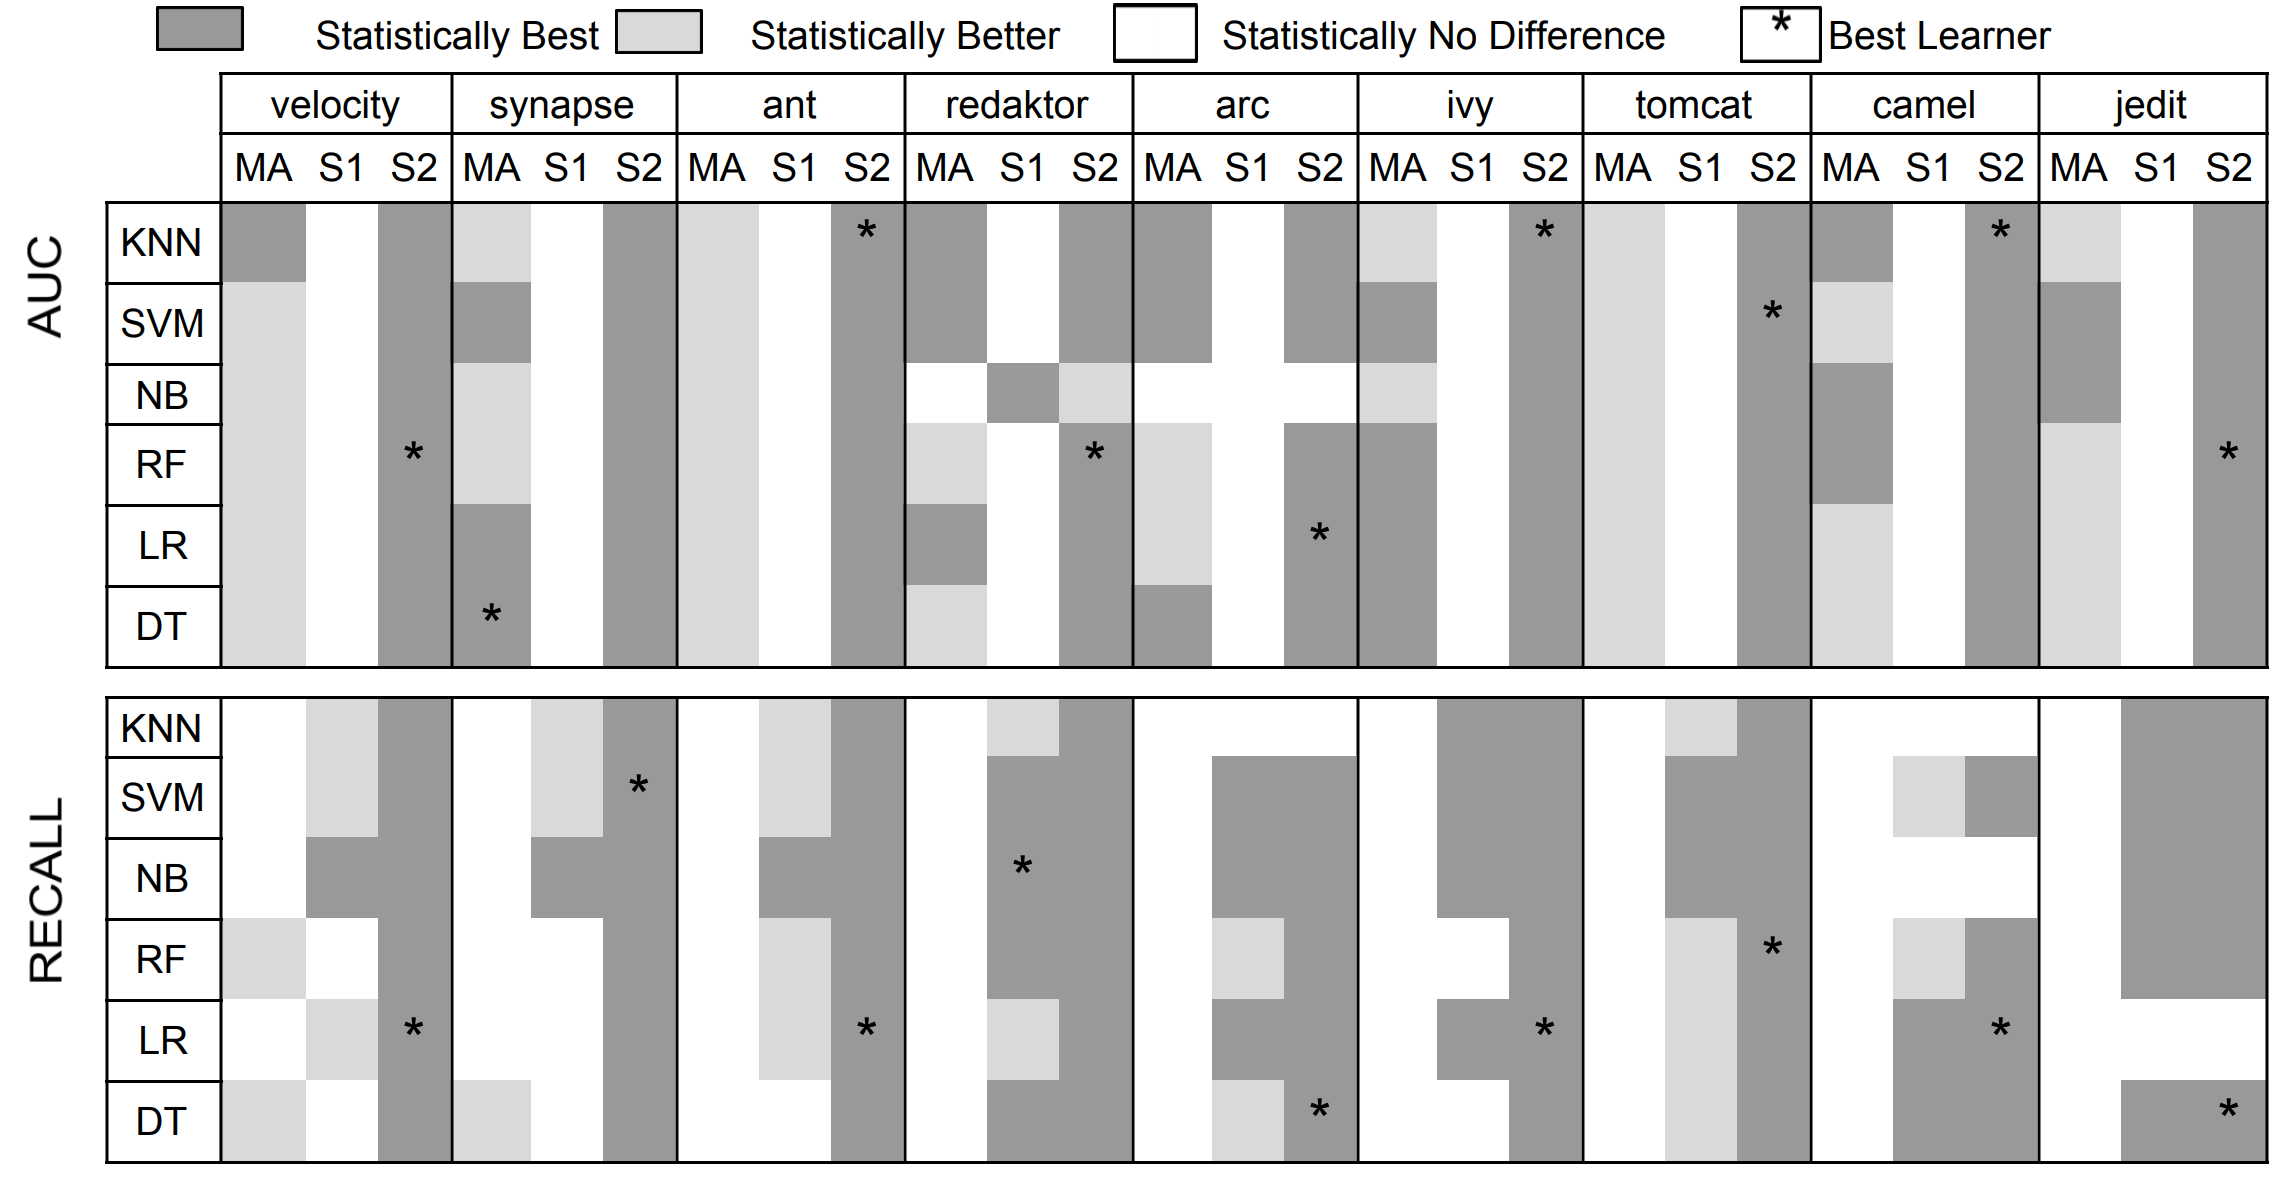
\includegraphics[width=0.9\linewidth,height=4.5cm ]{./fig/auc_maha.png}
%             \end{minipage}%
% \begin{minipage}{.49\linewidth}
%         \centering
%         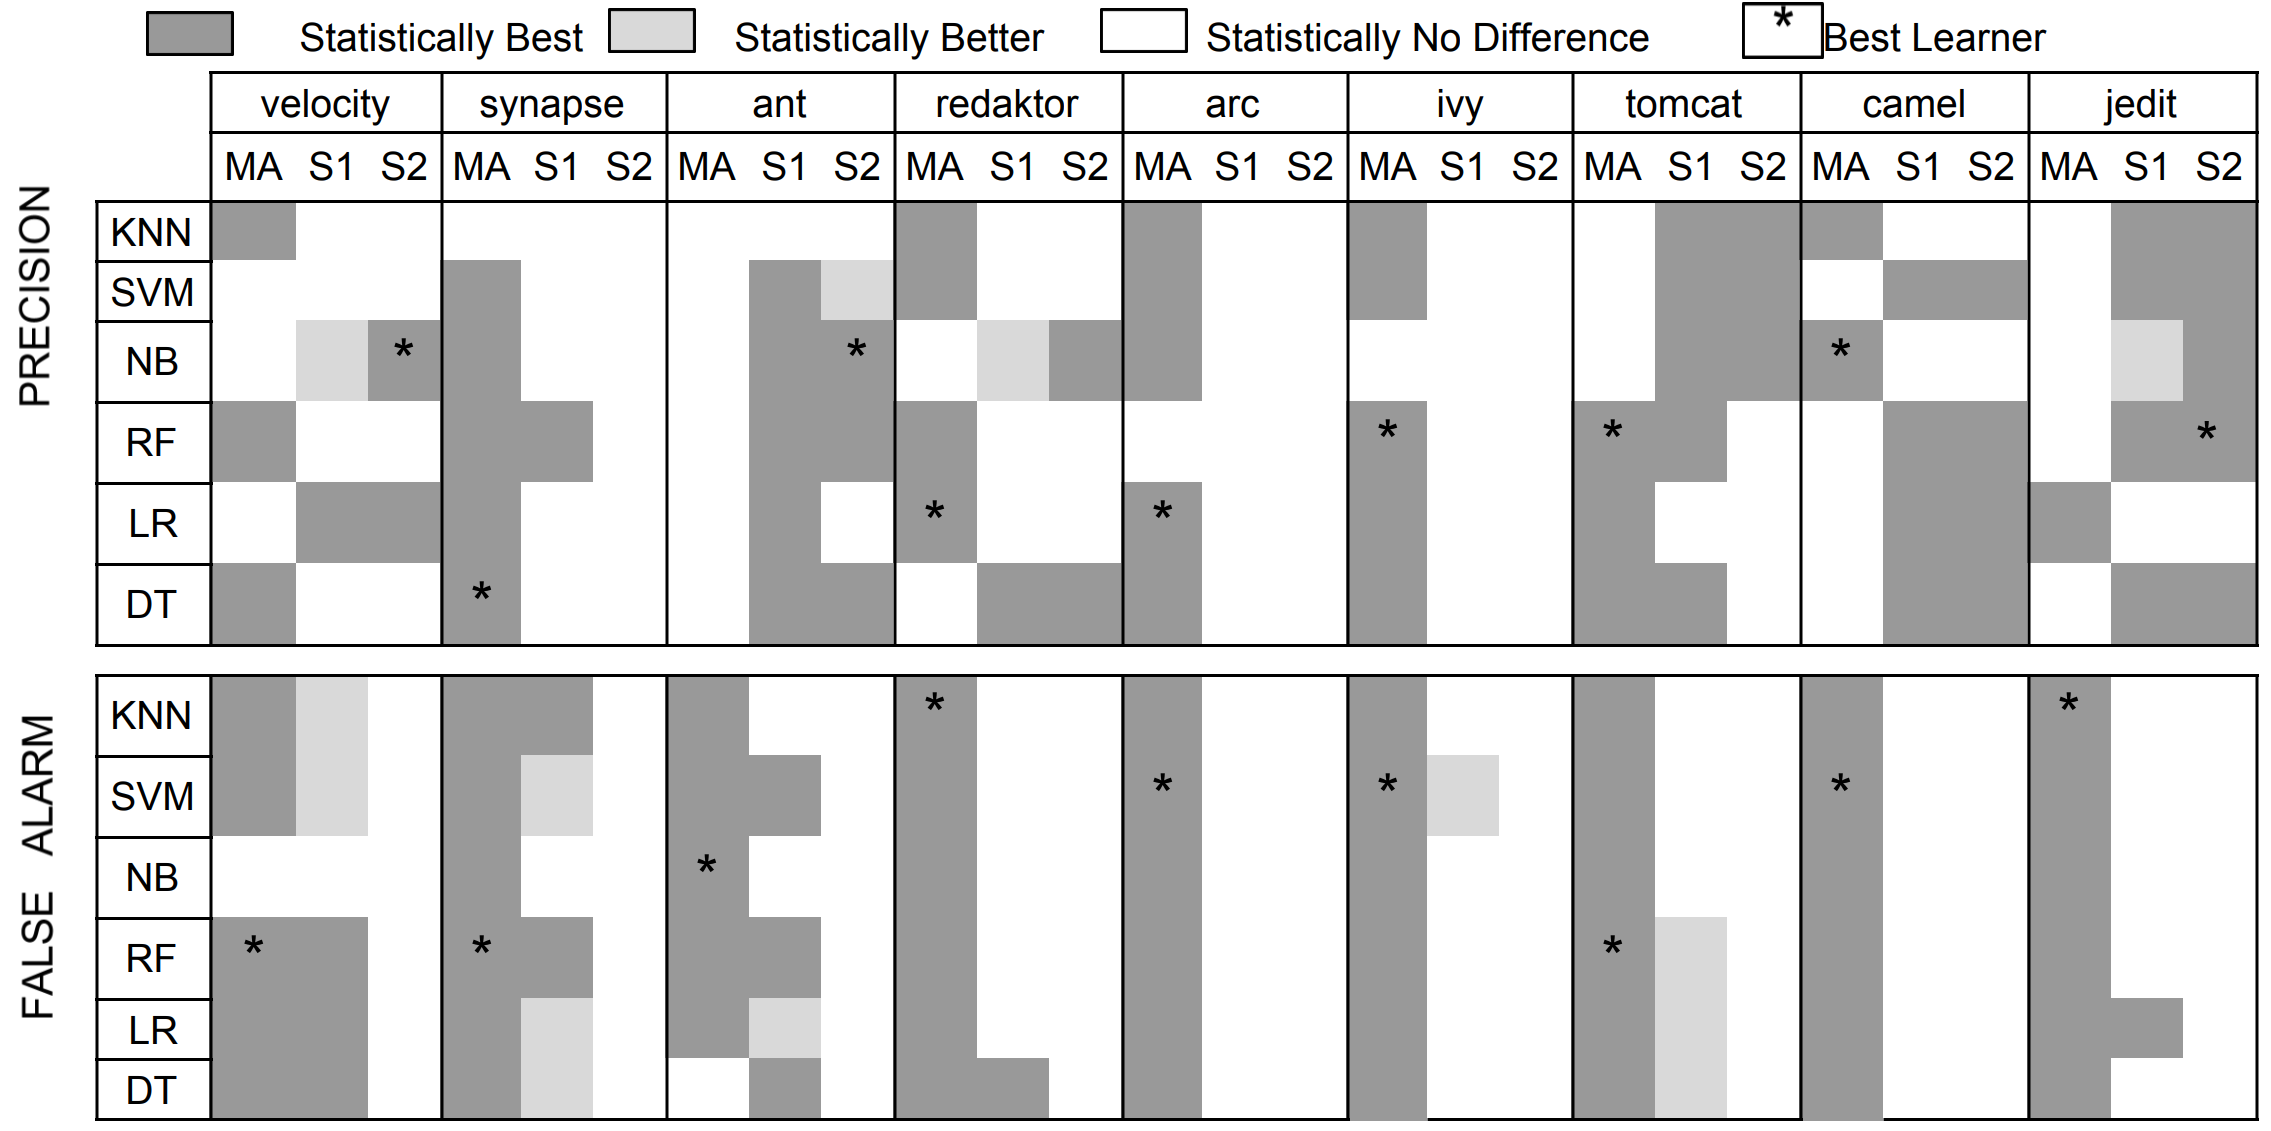
\includegraphics[width=0.9\linewidth,height=4.5cm]{./fig/prec_maha.png}
%     \end{minipage}%
%     \caption{Scott Knott analysis of MAHAKIL, SMOTE and SMOTUNED. The column headers are denoted as MA for MAHAKIL, S1 for SMOTE and S2 for SMOTUNED. $(\ast)$ Mark represents the best learner combined with its techniques}
%     \label{fig:s2_mahakil}
% \end{figure*}



% {\small \begin{center}
% AUC=8\%, \mathit{Recall}=+33; False Alarms= +18, precision=-6\%\%
% \end{center}
% }

% From the Scott-knott analysis as shown in Figure~\ref{fig:stats}, we selected out the best treatment in which a learner performed the best (represented with ``*'' in Figure~\ref{fig:stats}). We observed that:

% {\small\[\begin{array}{*{20}{c|c|c|c|c}}
%  & \multicolumn{4}{c}{\text{number of wins}}\\ 
%   {\text{Treatments}} & {\text{AUC}} & {\text{Recall}} & {\text{Precision}}& {\text{False Alarm}}\\
%   \hline
%   {\text{No-SMOTE}} & 0/9 & 0/9 & \textbf{5/9} & \textbf{9/9}  \\
%   {\text{SMOTE}}& 0/9 & 0/9 & 0/9 & 0/9 \\
%   {\text{SMOTUNED}}& \textbf{9/9} & \textbf{9/9} & 4/9  & 0/9 
% \end{array} \]}

% \noindent
% Similarly, we performed a Scott-knott analysis as described in Section \ref{sec:scott-knott} to compare MAHAKIL against {\sma} and {\smb}.  We found that:
% \[\begin{array}{*{20}{|c|c|c|c|c|}}
% \hline
%   {\text{Treatments}} & {\text{AUC}} & {\text{Recall}} & {\text{Precision}}& {\text{False Alarm}}\\
%   \hline
%   {\text{MAHAKIL}} & 1/9 & 0/9 & \textbf{6/9} & \textbf{9/9}  \\
%   {\text{SMOTE}}& 0/9 & 1/9 & 0/9 & 0/9 \\
%   {\text{SMOTUNED}}& \textbf{8/9} & \textbf{8/9} & 3/9  & 0/9  \\
% \hline
% \end{array} \]


% As mentioned above in Section \ref{sect:wcm}, all recall increases naturally incur the cost of larger false alarms.


% \textcolor{red}{The most recent technique introduced by Benning et al~\cite{bennin2017mahakil} is MAHAKIL which is based on chromosomal theory of inheritance. A reproduction package was not available, so, coded their methods from scratch (our replication package for that code is now online (Blinded for Review).}
% %\footnote{Available to download from https://github.com/ai-se/MAHAKIL_imbalance}
% \textcolor{red}{Their study reported that {\sma} performed better than all other previous imbalance techniques (techniques reported by Bennin et al.) for recall and false alarm and produced similar results against MAHAKIL for recall measure. That said, they advocate MAHAKIL sicne it was observed
% to have better  (i.e. lower) false alarm rates.}

% % \textcolor{red}{We find this to be highly unlikely as we know from Zhang's equation~\cite{zhang2007comments} that if recall is increased then false alarm would also increase. The other important factor, find to be missing was an automated method of tuning the parameters of an imbalance technique and thus we introduced {\smb} and compared the 2 methods.}

% \textcolor{red}{To show the increase in recall would also result in false alarm, we compared the MAHAKIL results against the {\sma}. As shown in figure (available from http://ibb.co/e02bmk), we observed that we are seeing about 30\% improvement on {\sma} over MAHAKIL. But this also resulted in the increment of false alarm, which is not desired. But we see MAHAKIL wins over {\sma} in terms of AUC in most cases.}

% \textcolor{red}{For the comparative analysis of {\smb} and MAHAKIL, please look at the results from Figure~\ref{fig:s2_mahakil}.
% %which is available from http://ibb.co/fGZBK5. 
% We observed that we are getting consistent improvement on {\smb} of about 30\% than MAHAKIL, and {\smb} also resulted in improved performance in terms of AUC.}

% For more details on the differences between (a)~{\sma} vs MAHAKIL, see http://ibb.co/e02bmk (this chart is not included here, for reasons of space), for {\smb} vs MAHAKIL, please see Figure~\ref{fig:s2_mahakil}

\begin{figure*}[!t]
\begin{minipage}{.5\linewidth}
\centering
        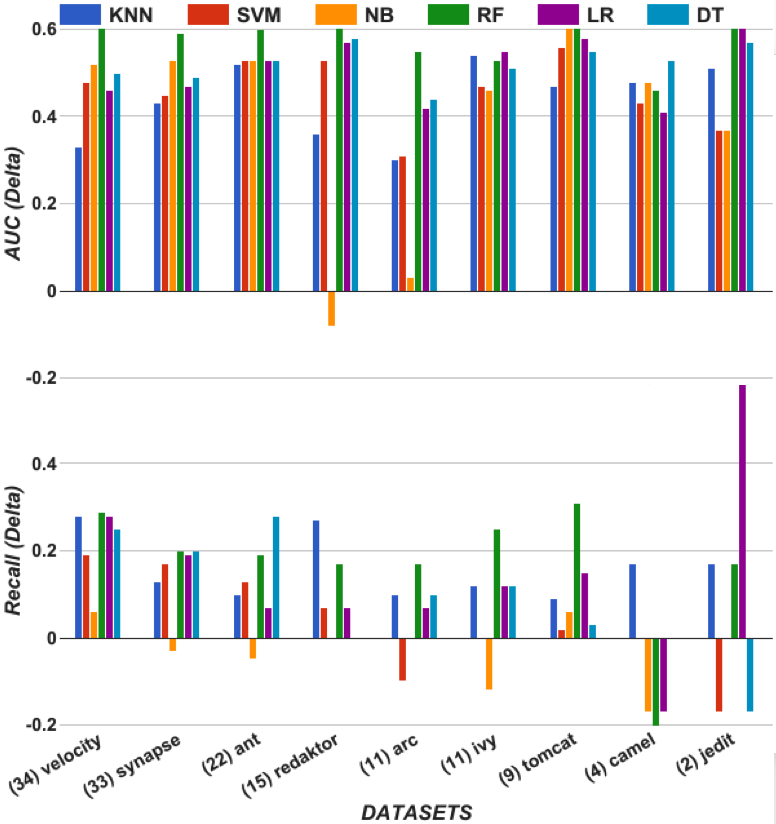
\includegraphics[width=.75\linewidth,keepaspectratio,trim=1cm 1cm 1cm 0cm]{./fig/AUC_auc1.png}
    \end{minipage}%
\begin{minipage}{.5\linewidth}
        \centering
        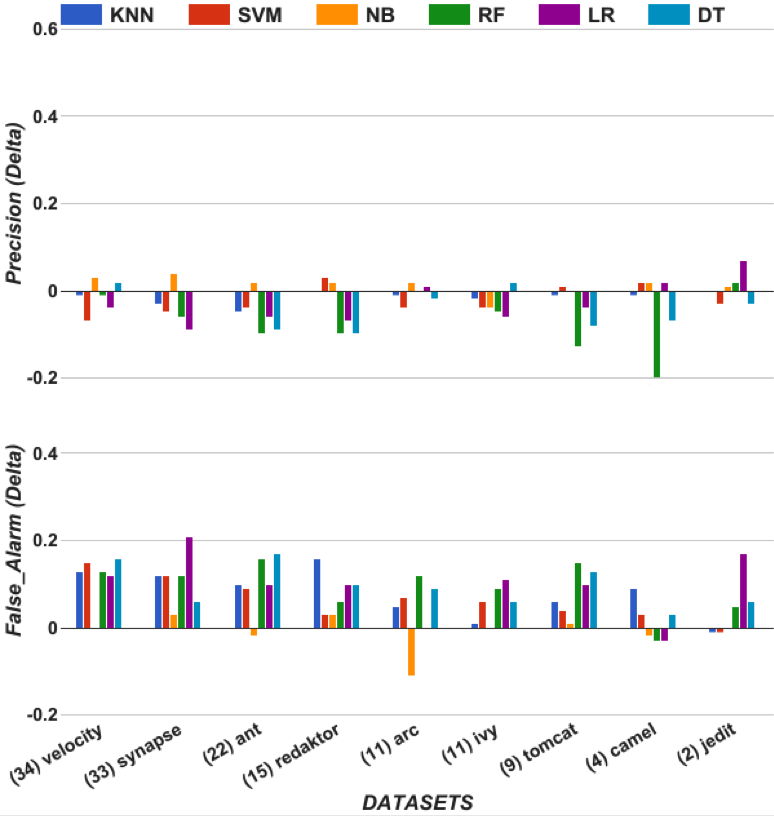
\includegraphics[width=.75\linewidth,keepaspectratio,trim=1cm 1cm 1cm 0cm]{./fig/AUC_prec.png}
    \end{minipage}%
    
    \caption{ SMOTUNED improvements over SMOTE. 
    \underline{{\bf Cross}}-Measure
    assessment (i.e., for each of these charts,
    optimize for \underline{{\bf AUC}}, then test for
    performance measure $M_i$).  Same format as
    Figure~\ref{fig:tuned}.}
    \label{fig:auc22}
\end{figure*}

\section{Threats to Validity}
\label{sect:validity}

As with any empirical study, biases can affect the final
results. Therefore, any conclusions made from this work must consider the following issues in mind.

\textbf{\textit{Order bias}}: With each data set how data samples are distributed in training and testing set is completely random. Though there could be times when all good samples are binned into training and testing set. To mitigate this order bias, we run
the experiment 25 times by randomly changing the order of the data samples each time.

\textbf{\textit{Sampling bias}} threatens any classification experiment, i.e., what matters there may not be true here. For example, the data sets used here comes from the SEACRAFT repository and were supplied by one individual. These data sets have used in various case studies by various researchers~\cite{he2012investigation,peters2013better,peters2013balancing,turhan2013empirical}, i.e., our results are not more biased than many other studies in this arena.
That said, our nine open-source data sets   are mostly from Apache. Hence
it is an open issue if our results hold for
 proprietary projects and open source projects from other sources.

% \textbf{\textit{Learner bias}}: For building the defect predictors in this
% study, we selected each learner with default parameters like k=8 in $k$-NN, entropy as split criteria in RF, and DT. The above predefined parameters have been used in the conclusions made by other studies~\cite{ghotra2015revisiting,tantithamthavorn2016automated}. 

\textbf{\textit{Evaluation bias}}: In terms of evaluation bias,
our study is far less biased than many other ranking studies.  As shown by our sample of
22 ranking studies in
Table~\ref{tbl:survey2}, 19/22 of those prior studies used {\em fewer} evaluation criteria
than the four reported here (AUC, recall, precision and false alarm). 

The analysis done in RQ4 could be affected by some other settings which we might not have considered since the reproduction package was not available from the original paper~\cite{bennin2017mahakil}.
That said, there is another more subtle evaluation bias arises in the Figure~\ref{fig:tuned}. The four plots of that figure are four {\em different} runs of our  {\em within-measure assessment rig}
(defined in \tion{wcm}). Hence, it is reasonable to check what happens when (a)~one
evaluation criteria is used to control {\smb}, and (b)~the results are assessed
using all four evaluation criteria. 
Figure~\ref{fig:auc22} shows the results of such a {\em cross-measure assessment rig} where AUC was used to control {\smb}. We note that the results in this figure are very similar to Figure~\ref{fig:tuned}, e.g., the precision deltas aver usually tiny, and false alarm increases are usually smaller than the associated recall improvements. But there are some larger improvements in Figure~\ref{fig:tuned}
than Figure~\ref{fig:auc22}. Hence, we recommend cross-measure assessment only if CPU is critically restricted. Otherwise, we think {\smb} should be controlled by whatever is the downstream evaluation criteria
(as done in the within-measure assessment rig of Figure~\ref{fig:tuned}.)



\section{Conclusion}
\label{sect:conclusion}





Prior work on ranking studies tried to improve software analytics by selecting better learners.
Our results show that there may be {\em more} benefits in exploring data pre-processors like {\smb} because we found  that no  learner  was  usually  
``best''  
across all  data  sets  and  all  evaluation  criteria. On the other hand, across the same data sets,
{\smb} was  consistently  used  by  whatever  learner  was  found  to  be ``best'' in the  AUC/recall results. On the other hand, for the precision and false alarm results, there was little evidence against the use of {\smb}. That is, creating better training data  (using techniques like {\smb}) may be  more important than  the  subsequent  choice  of a classifier. To say that another way, at least for defect prediction, ``better data'' is  better than ``better
data miners''.


As to specific recommendations, we suggest that any prior ranking study  which did not  study the effects of data pre-processing needs to be analyzed again. Any future such ranking study should include a {\sma}-like
 pre-processor. {\sma} should not be used with its default parameters.
 For each new data set, {\sma} should be used with some automatic parameter tuning tool in
order to find the best parameters for that data set. {\smb} is one of the examples of parameter tuning. Ideally, {\smb} should be tuned using the evaluation criteria used to assess the final predictors. However, if there is not enough CPU to run {\smb} for each new evaluation criteria, {\smb} can be tuned using AUC.
% We conjecture that {\smb}
% is best viewed as a   {\em signal amplifier} for regions of the data where the quality signal is weak  (e.g., sparse regions with very little data between far-flung outliers).

% One surprise from our results was that the performance improvements associated with {\smb} were not substantially different between balanced and unbalanced data sets.
%  {\sma} was originally proposed as a method to correct class imbalance, e.g., when the target class is only a small fraction of the instances in the training data.
%  Yet our results show that {\sma} (and {\smb}) is also useful for balanced data sets (and best results come from automatically tuning the control parameters of {\sma}). 



% \section*{Acknowledgements}
% The work is partially funded by
% %NSF awards \#1506586  and \#1302169.
% funding source (blinded for review).

\balance

%\bibliographystyle{abbrv}

\bibliographystyle{ACM-Reference-Format}
%\medskip
 
\documentclass[sigconf,review, anonymous]{acmart}

\usepackage{graphicx}
\usepackage[colorinlistoftodos]{todonotes}
\usepackage{blindtext, graphicx}
\usepackage{hyperref}
\usepackage{caption}
\usepackage{float}
\usepackage{balance}
\usepackage{listings}
\renewcommand\thesection{\arabic{section}.}
\renewcommand\thesubsection{\thesection\arabic{subsection}}
\usepackage{amsmath}
\usepackage{tikz}
\usepackage{comment}
\usepackage{framed}
\usepackage{multirow}
\usepackage{rotating}
\usepackage{bigstrut}
\usepackage{color}
\usepackage{eqparbox}
\usepackage{graphics}
\usepackage{colortbl}
\usepackage{paralist}
\usepackage{algorithm}
\usepackage{algorithmicx}
\usepackage{algpseudocode}
\usepackage{mathptmx} 
\usepackage{picture}
\usepackage[shortlabels]{enumitem}
\usepackage{url}

\newcommand{\bi}{\begin{itemize}[leftmargin=0.4cm]}
	\newcommand{\ei}{\end{itemize}}
\newcommand{\be}{\begin{enumerate}}
	\newcommand{\ee}{\end{enumerate}}

\usepackage{tabularx}
\usepackage{colortbl}
\usepackage{hhline}
\usepackage[export]{adjustbox}
\definecolor{lightgray}{gray}{0.8}
\definecolor{darkgray}{gray}{0.6}
\definecolor{lavenderpink}{rgb}{0.98, 0.68, 0.82}
\definecolor{celadon}{rgb}{0.67, 0.88, 0.69}
\renewcommand{\algorithmicrequire}{\textbf{Input:}}
\renewcommand{\algorithmicensure}{\textbf{Output:}}
%%% graph
\newcommand{\crule}[3][darkgray]{\textcolor{#1}{\rule{#2}{#3}}}

\newcommand{\quart}[4]{\begin{picture}(80,4)%1
	{\color{black}\put(#3,2){\circle*{4}}\put(#1,2){\line(1,0){#2}}}\end{picture}}

\definecolor{Gray}{gray}{0.95}
\definecolor{LightGray}{gray}{0.975}

\definecolor{steel}{rgb}{.11, .11, .7}
\definecolor{Gray}{rgb}{0.88,1,1}
\definecolor{Gray}{gray}{0.85}
\usepackage[framed]{ntheorem}
\usetikzlibrary{shadows}
\theoremclass{Lesson}
\theoremstyle{break}

% inner sep=10pt,
\tikzstyle{thmbox} = [rectangle, rounded corners, draw=black,
fill=Gray!40,  drop shadow={fill=black, opacity=1}]
\newcommand\thmbox[1]{%
	\noindent\begin{tikzpicture}%
	\node [thmbox] (box){%
		\begin{minipage}{.94\textwidth}%
		\vspace{0mm}#1\vspace{0mm}%
		\end{minipage}%
	};%
	\end{tikzpicture}}

\let\theoremframecommand\thmbox
\newshadedtheorem{lesson}{Result}
\newcommand{\tion}[1]{{\S}\ref{sect:#1}}

\setcopyright{rightsretained}


\acmConference[FSE'2017]{ACM SIGSOFT SYMPOSIUM ON THE FOUNDATIONS OF SOFTWARE ENGINEERING}{September 2017}{PADERBORN, GERMANY} 
\acmYear{2017}
\copyrightyear{2017}

\acmPrice{15.00}


\begin{document}

%\pagestyle{plain}

\title{Reanalyzing Defect Prediction - Can Not Assess Learners Without a Pre-Tuning Study}

\author{Amritanshu Agrawal}
\affiliation{%
  \institution{North Carolina State University}  \city{Raleigh}
  \state{North Carolina, USA}}
\email{aagrawa8@ncsu.edu}

\author{Tim Menzies}
\affiliation{%
  \institution{North Carolina State University}  \city{Raleigh}
  \state{North Carolina, USA}}
\email{tim@menzies.us}



\begin{abstract}
Software Engineering (SE) is complex. Hence, the data associated with SE projects 
can also be complex and noisy. Preprocessing methods are employed to make the data 
simple and useful for any software analytics. But the continuous trend observed 
is that classification techniques are used without giving much thought to various 
preprocessing methods. For example, defect data sets are often ``imbalanced''; 
i.e. the defects are a small minority of the entire set of examples. Due to that 
performance of such learners could be highly affected.

One way to handle imbalance is the SMOTE procedure (Synthetic Minority Oversampling Technique) which is a pre-processing filter, to
throw away random examples of the majority
class while at the same time, synthesizing
more examples 
of the minority class (a.k.a. making up defect data). 
SMOTE is controlled by numerous
parameters. Off-the-shelf SMOTE~1  uses the default
parameter settings while our tuned SMOTE~2 algorithm
uses parameters set found by a search-based SE technique
called differential evolution. 

In studies with SMOTE~1 and SMOTE~2 performed on
 9 defect data sets, we find that SMOTE~1 may or may not be useful, depending on the evaluation goal. For example,
 for precision the results were mixed-- sometimes better sometimes worse.
On the other hand, the tunings
used in SMOTE~2 lead to dramatic improvements in  AUC (pf, recall) and these were 
much better than SMOTE~1. And larger improvements were seen in recall results using SMOTE~2 (and here again SMOTE~2 performed better than SMOTE~1).

Hence, we conclude that (a)~making up defect data with SMOTE~2 is useful when trying to improve performance on certain goals. Also, (b)~it is best {\em not} to use the default parameters of off-the-shelf SMOTE~1. And (c)~which preprocessing methods to use should be
given equally importance as to which learners to employ.
\end{abstract}

%\keywords{
%Performance Prediction, SBSE, Sampling, Rank-based method}
\keywords{defect prediction, classification, SMOTE, search based software engineering, imbalance data, preprocessing}

\maketitle

%\category{H.4}{Software Engineering}{Defect Prediction}
%A category including the fourth, optional field follows...
%\category{D.2.8}{Software Engineering}{Metrics}[complexity measures, performance measures]

%\terms{Theory}


\section{Introduction}

Time and manpower being finite resources, it
makes sense to assign personnel and/or resources to areas of
a software system with a higher probable quantity of defects. Current defect prediction work focuses on (i) estimating the number of defects remaining in software systems, (ii) discovering defect associations, and (iii) classifying the defect-proneness of software components, typically into two classes defect-prone and not defect-prone. 

% There has been vast amount of studies done to find the best defect prediction performing model which is related to third type of problem. But literature suggests, that no single prediction technique dominates and making sense of the many prediction results is hampered by the use of different data sets, data pre-processing, validation schemes and performance
% statistics. We highly agree to this given so many variations available in the data and there are so many classification techniques available like Statistical, Clustering, Rule-Based, Neural Networks, Nearest Neighbour, Support Vector Machines, Decision trees, ensemble methods, to name a few.

This paper deals with the third type of problem for code metrics (especially, the 
CK object-oriented metrics~\cite{chidamber1994metrics}).
Our task is to classify the defect-proneness of software components, typically into two classes, defective and not defective.

One issue with this kind of research is deciding
which data mining algorithm is best for a particular
data set. In a comparative study of numerous
learners for defect prediction, Ghotra et al.~\cite{ghotra2015revisiting} recommended six learners: Naive Bayes, Logistic regression, Support Vector Machines, Nearest Neighbor, decision trees and Random forest. One small drawback with their
work was that they did not study the effects of class imbalance for such models.
This is an important factor
since most software systems have less than 20\% defective classes. Accordingly, this paper
explores the Ghotra et al. learners using data
sets that have an increasingly large imbalances
in the frequency of the defect class. Specially, we use data sets where the percent
of defective classes
range down to 4\%. 

Handling the class imbalance is another issue which comes 
under the preprocessing part. We found this to be an important aspect in defect prediction which is shown in \tion{results} The level of imbalance is not the only factor that hinders
the performance of the classifiers, and other factors
such as the degree of data overlapping (represented
as duplicates) among the classes also leads to the decrease in performance of
learning algorithms. As stated by Lopez et al.~\cite{lopez2014importance,lopez2012analysis} there
are other problems: dataset shift (training and test
data follow different distributions), distribution of the
cross validation data, small disjuncts, the lack of density
or small sample size, the class overlapping, the
correct management of borderline examples or noisy
data. Many of these problems are related to how to
measure these data characteristics and the quality of
data. For instance, Van et al.~\cite{van2009knowledge}
have looked into how the level of noise in data (quality) impact the performance of the classifiers. This makes a necessary argument to study preprocessing filters and how it can affect the performance of classifiers. In this paper we have tackled only the class imbalance problem.

The imbalance problem is known to affect
many machine learning algorithms such as decision tress,
neural networks or support vectors machines \cite{japkowicz2002class}. In this paper, we evaluate the performance of using a class balancing technique (which we are calling standard SMOTE~1\cite{chawla2002smote}) against running all classifiers on the imbalanced datasets without SMOTE~1. What was observed is even after using SMOTE, there was stability problem as class goes more minor and minor. A general trend should have been that performance should increase as target class goes more minor and minor. To study this instability in results, we propose a search-based optimizer (differential evolution, or DE~\cite{storn1997differential}) to tune the parameters of SMOTE to get the best results out of them.
We call this tuned version SMOTE~2.

In this context, we explore two research questions:  
 
  \textbf{RQ1}: \textbf{Is standard ``off-the-shelf'' SMOTE~1 preprocessing method important for defect prediction?} 

 \begin{lesson}For defect data, SMOTE~1 has little effect on 
 precision, modest improvements for AUC (pf, recall) and largest improvements in recall.
 \end{lesson}

 \textbf{RQ2}: \textbf{Can tuning SMOTE~1 (SMOTE~2) achieve better results?} 
 
 \begin{lesson}For defect data, SMOTE~2  
 offered  large  improvements over SMOTE~1 for recall
 and dramatic improvements for AUC (pf, recall).
 \end{lesson}
 
 \textbf{RQ3}: \textbf{Do different data sets
      need different configurations with SMOTE~2?} 
 
 \begin{lesson}DE finds different ``best'' parameter settings for SMOTE for different data sets. Hence reusing tunings  suggested  by  any other  previous study  for any dataset is \underline{{\em not}} recommended. Instead,  it is better to
      use automatic tuning  methods  to find the best tuning parameters for the current data set.
 \end{lesson}
   \textbf{RQ4}: \textbf{Is tuning extremely slow?} 
 
 \begin{lesson}Tuning with DE makes training three to five times slower, but the improvements which we get for AUC and recall is quite advantageous.
 \end{lesson}
 
 \begin{figure*}[t!]
\renewcommand{\baselinestretch}{0.8}\begin{center}
{\scriptsize
\begin{tabular}{c|l|p{4.0in}}
amc & average method complexity & e.g. number of JAVA byte codes\\
\hline
avg, cc & average McCabe & average McCabe's cyclomatic complexity seen
in class\\
\hline
ca & afferent couplings & how many other classes use the specific
class. \\
\hline
cam & cohesion amongst classes & summation of number of different
types of method parameters in every method divided by a multiplication
of number of different method parameter types in whole class and
number of methods. \\
\hline
cbm &coupling between methods & total number of new/redefined methods
to which all the inherited methods are coupled\\
\hline
cbo & coupling between objects & increased when the methods of one
class access services of another.\\
\hline
ce & efferent couplings & how many other classes is used by the
specific class. \\
\hline
dam & data access & ratio of the number of private (protected)
attributes to the total number of attributes\\
\hline
dit & depth of inheritance tree &\\
\hline
ic & inheritance coupling & number of parent classes to which a given
class is coupled (includes counts of methods and variables inherited)
\\
\hline
lcom & lack of cohesion in methods &number of pairs of methods that do
not share a reference to an case variable.\\
\hline
locm3 & another lack of cohesion measure & if $m,a$ are the number of
$methods,attributes$
in a class number and $\mu(a)$ is the number of methods accessing an
attribute,
then
$lcom3=((\frac{1}{a} \sum, j^a \mu(a, j)) - m)/ (1-m)$.
\\
\hline
loc & lines of code &\\
\hline
max, cc & maximum McCabe & maximum McCabe's cyclomatic complexity seen
in class\\
\hline
mfa & functional abstraction & number of methods inherited by a class
plus number of methods accessible by member methods of the
class\\
\hline
moa & aggregation & count of the number of data declarations (class
fields) whose types are user defined classes\\
\hline
noc & number of children &\\
\hline
npm & number of public methods & \\
\hline
rfc & response for a class &number of methods invoked in response to
a message to the object.\\
\hline
wmc & weighted methods per class &\\
\hline
\rowcolor{lightgray}
nDefects & raw defect counts & Numeric: number of defects found in post-release bug-tracking systems.\\
\rowcolor{lightgray}
defects present? & Boolean: if {\em nDefects} $>0$ then {\em true} else {\em false}
\end{tabular}
}
\end{center}
\caption{OO code metrics used for all studies in this paper.
Last lines, shown in \textcolor{gray} denote the dependent variables.}
\label{fig:ck}
\end{figure*}

Hence, we will conclude that if SMOTE is used,
then it is best {\em not} to use the off-the-shelf tunings. Rather, it is best to employ some search-based
SE method to find the tunings that work best for the
particular data set under study.

The rest of this paper is structured as follows.
\tion{review} gives an overview of ways in which software defect prediction has been done before. \tion{motivation} argues why balancing the minority class is important.
What is SMOTE and how it has been used before is talked in \tion{smote}. Advantages
of tuning is mentioned in \tion{tune}
and the experimental setup of this paper is discussed in \tion{experiment}
We have answered above research questions in
\tion{results} This is followed by a discussion on the validity of our results 
and a section describing our conclusions.

% \item \textbf{RQ3}: \textbf{Should SMOTE be used ``off-the-shelf'' with their default tunings?}

 

%We created a python package generalised to run any CK metrics based dataset and compare results against 6 learners. Since the classes are imbalanced we used SMOTE~\cite{chawla2002smote} (only on Training Data) which is a synthetic minority over-sampling technique.

%The remainder of the paper is organized as follows. Section \ref{review} gives a brief related work on defect prediction. Section \ref{motivation} talks about why there is a need to balance the data. Since we found astonishing results with smote, section \ref{smote} talks about SMOTE in defect prediction. Experimental setup is provided in section \ref{experiment}. Results are discussed in Section \ref{results}. Threats to validity section is discussed in section \ref{validity}. Final conclusion is being discussed in section \ref{conclusion}. And section \ref{future} talks about our future work.

\section{Related Work}
\label{sect:review}

Much prior work has estimated number of defects remaining in software systems~\cite{hall2012systematic} using statistical approaches, capture-recapture 
(CR) models, and detection profile methods (DPM)~\cite{song2011general} or
association rule mining~\cite{song2006software}. A variety of approaches have been proposed to tackle the problem of classifying the defect-proneness of software components. It is heavily relied on diverse information, such as code metrics~\cite{d2010extensive,menzies2007data, nagappan2006mining,shepperd2014researcher,Menzies2010} (lines of code, complexity), process metrics~\cite{hassan2009predicting} (number of changes, recent activity) or previous defects~\cite{kim2007predicting}.

Bird et al.~\cite{bird2009putting} indicate that it is possible to predict which components are likely locations of
defect occurrence using a component's development history,
and dependency structure. Two key properties of software components
in large systems are dependency relationships (which components
depend on or are dependent on by others), and development
history (who made changes to the components and
how many times). Thus we can link software components
to other components a) in terms of their dependencies, and
also b) in terms of the developers that they have in common. Prediction models based on the topological properties
of components within them have proven to be quite
accurate~\cite{zimmermann2008predicting}.

By keeping change logs of the most recently or frequently changed files are the most probable source of future defects~\cite{hall2012systematic, catal2009systematic}. These mentioned papers compared various code metrics like CK  metrics  suite,  
McCabes  cyclomatic  complexity, Briands coupling metrics, code metrics, 
dependencies between  binaries. The CK metrics aim at measuring whether a 
piece of code follows OO principles. It contains a check of these OO design 
attributes which are explained in Figure \ref{fig:ck}. CK metrics is a set
of metrics and it has added advantage than other OO and static code attributes metrics~\cite{d2010extensive}. 

There are other added advantage that comes with CK metrics as they are  simple  to  compute. They have been popular in past covering research papers about twice (49\%) 
as more traditional source code metrics (27\%) or process metrics (24\%)~\cite{radjenovic2013software}. 

There has been vast amount of studies done to find the best defect prediction performing model. But literature suggests, that no single prediction technique dominates and making sense of the many prediction results is hampered by the use of different data sets, data pre-processing, validation schemes and performance
statistics. We highly agree to this given so many variations available in the data 
and there are so many classification techniques available like Statistical, Clustering, Rule-Based, Neural Networks, Nearest Neighbour, Support Vector Machines, Decision trees, ensemble methods, to name a few.

Different data preprocessing has been proved
to improve the performance of defect prediction models by
Menzies et al.~\cite{menzies2007data}. Jiang et al.~\cite{jiang2008can} evaluate the impact of
log transformation and discretization on the performance
of defect prediction models, and find different modelling
techniques ``prefer'' different transformation techniques. For
instance, Naive Bayes achieves better performance on discretized
data, while logistic regression achieves better performance
for both. Peters et al.~\cite{peters2013better} propose different filters; and Li et al.~\cite{li2012sample} propose
to use sampling. Nam et al.~\cite{nam2013transfer} propose to transform both
training and testing data to the same latent feature space,
and build models on the latent feature space.  High-dimensional feature always accompanies with the class-imbalance. Too many variables in the data
can result in the ``curse of dimensionality''~\cite{friedman1997bias}. The Feature Selection is a common method that can
reduce features and sampling can balance the diversity of
class instance numbers~\cite{yin2015empirical}, in turn improving the performance of defect prediction.

To tackle the variations available among classifiers, some studies suggested to tune the learners to find the best parameter settings~\cite{tantithamthavorn2016automated, fu2016tuning}.  According to them every dataset comes with different attributes and with different configurable learners, and we can not use a parameter settings found out by previous studies. Every time a defect prediction learner is used it is recommended to find automatic ways to tune them. And in such cases, automatic 
methods are required to do hyperparameter optimization~\cite{agrawal2016wrong, fu2016tuning}. This was the motivation to use an automatic method like DE to
tune the settings of SMOTE.

In terms of the paper with most influenced work,
our experimental methods are informed 
by  Ghotra et al.~\cite{ghotra2015revisiting} on ``Revisiting the impact of classification techniques on the performance of defect prediction models''. To 
compare  the  performance  of  defect prediction  models,  they  used  the  Area  Under  the receiver operating characteristic Curve (AUC), which plots  the  false  positive  rate  against  the  true  positive rate. We denote this AUC (pf,pd). 
They ran the Scott-Knott test to group classification techniques into statistically distinct ranks. After running these evaluation criteria, they concluded that Naive Bayes, Logistic regression, Support Vector Machines, Nearest Neighbor, decision tree and Random forest performs the best depending on various datasets. Accordingly, 
we use these learners in this paper.

\section{Motivation}
\subsection{Preprocessing to balance the class}
\label{sect:motivation}

Class imbalance learning refers to learning from data sets that exhibit significant imbalance among or within classes. Class imbalance  is concerned with the situation in which some classes of data are
highly under-represented compared to other classes~\cite{he2009learning}. By convention,
the under-represented class is called the {\em minority} class,
and correspondingly the class having the larger size is called the
{\em majority} class. In this paper, we say that imbalance is worse when the percent frequency of
the minority class {\em decreases}. That is,
{\em minority=5\%} is worst than {\em minorty=20\%}.

Misclassifying an example from the minority class is usually more costly. For software defect prediction, due to the nature of the problem, the defect case is much less likely to happen than the non-defect case.  The failure of finding a defect could degrade software quality greatly (since more bugs
are delivered to the client). Hence,
our learning objective can be generally described
as ``obtaining a classifier that will provide higher performances for the minority class''.

Numerous methods have been proposed to tackle class
imbalance problems at data and algorithm levels. Data-level include a variety of resampling techniques, manipulating training data to rectify the skewed class distributions, such as random oversampling, random undersampling, and SMOTE~\cite{estabrooks2004multiple}. Algorithm-level methods address class imbalance by
modifying their training mechanism directly with the 
goal of better accuracy on the minority class, including cost-sensitive learning algorithms ~\cite{he2009learning}.
Algorithm-level methods require specific treatments for different
kinds of learning algorithms, which hinders their use
in many applications, because we do not know in advance
which algorithm would be the best choice in most cases. In addition to the aforementioned data-level and algorithm-level solutions, ensemble learning has become another major category of approaches to handle imbalanced data by combining multiple classifiers, such as SMOTEBoost~\cite{chawla2003smoteboost}, and
AdaBoost.NC~\cite{wang2010negative}. To 
the best of my knowledge, none of these methods have  thoroughly investigated the class imbalance problem.

Hall et al.~\cite{hall2012systematic} found that models based on C4.5 seem to underperform if they have imbalanced data while Naive Bayes and Logistic regression perfrom relatively better. 
Their general recommendation is not use
imbalanced data.  

Yu et al.~\cite{yuperformance} validated the Hall et al. results and concluded that the
performance of C4.5 is unstable on imbalanced datasets. They studied the stability issues due to  class imbalance and found out that Random Forest and Naive Bayes are the most stable. They generated synthetic datasets from the original one to build class imbalance datasets. This could be affected by random sampling 
so this may not be the ideal way to build imbalanced datasets. They also used default set of parameters but wanted to study the effects of tuning classifiers as well as mentioned to use techniques like SMOTE for class imbalance.

Wang et al.~\cite{wang2013using} studied various undersampling and oversampling technique and compared the results with Naive Bayes and random forest. Other interesting finding was to use AdaBoost.NC which have better performance than the rest while others are planning to use SMOTE~\cite{gray2009using} in future studies. Yan et al.~\cite{yan2010software} performed fuzzy logic and rules to overcome the imbalance problem only to work with Support Vector Machines. 

Pelayo et al.~\cite{pelayo2007applying} studied the effects of percentage of oversampling and undersampling done. They found out that different percentage of each helps improve the accuracies of decision tree learner for defect prediction using CK metrics. Menzies et al.~\cite{menzies2008implications} undersampled the non-defect class to balance training
data, and checked how little information was required to learn a defect predictor. They found that throwing away data does not degrade the performance of Naive Bayes and C4.5 decision trees, and instead improves the performance of C4.5. Some other papers also showed the usefulness of resampling based on different learners~\cite{pelayo2007applying, pelayo2012evaluating, riquelme2008finding}.

\subsection{Advantages of SMOTE}
\label{sect:smote}

There have been various oversampling and undersampling techniques available. And SMOTE~\cite{chawla2002smote} has become increasingly popular in recent times. SMOTE works by creating a new minority-class sample at a random point along the line
segments joining any/all of the k minority class nearest neighbors. Depending upon the
amount of over-sampling required, neighbors from the k nearest neighbors are randomly
chosen. Our implementation currently uses 5 nearest neighbors for SMOTE~1 method and for SMOTE~2, DE finds the best k. creates new instances using the selected instances and their neighbors. Synthetic samples
are generated in the following way: Take the difference between the feature vector (sample)
under consideration and its nearest neighbor. Multiply this difference by a random number
between 0 and 1, and add it to the feature vector under consideration. This causes the
selection of a random point along the line segment between two specific features.

Pears et al.~\cite{pears2014synthetic} used SMOTE to study software build outcomes. They observed
that classification accuracy steadily improves after creating synthetically approximately 900 instances of builds that have been fed to the classifier. Tan et al.~\cite{tan2015online} investigated on online defect prediction for imbalance data. They studied resampling techniques and found improvement in precision by 12.2 - 89.5\% or 6.4 - 34.8 percentage points. Removing testing-related changes can improve F1 by 62.2 - 3411.1\% or 19.4 - 61.4 percentage points. while achieving a comparable precision.

Pelayo~\cite{pelayo2007applying} found out that by using SMOTE, there was no improvement but other resampling strategies like trial-and-error, showed promising results by arriving at the highest geometric mean accuracies. Kamei et al.~\cite{kamei2007effects} evaluated the effects of SMOTE applied to only four fault-proneness models
(linear discriminant analysis, logistic regression
analysis, neural network and classification tree) by
using two module sets of industry legacy software. They reported SMOTE improved the prediction performance of the linear and logistic models, while neural network and classification tree models did not
benefit from it. In~\cite{van2007experimental} it is identified that classifier performance is improved with SMOTE, but individual learners respond differently on sampling. We will be studying many more models and will show that SMOTE does help in all prediction models depending on tuning goal.

\subsection{Importance of Tuning}
\label{sect:tune}

The impact of tuning is well understood in the theoretical machine learning literature~\cite{bergstra2012random}.  When we tune a
data miner, what we are really doing is changing how a learner applies its
heuristics. This means tuned data miners use different heuristics, which means
they ignore different possible models, which means they return different models;
i.e. \textit{how} we learn changes \textit{what} we learn.

Yet issues relating to
tuning are poorly addressed in the software analytics literature. But there are studies done by so many researchers showing big advantages. Fu et al.~\cite{fu2016tuning} surveyed hundreds of recent SE papers in the area
of software defect prediction from static code attributes. They found that most SE
  authors do not take steps to explore tunings (rare exception:~\cite{tantithamthavorn2016icse}). For example, Elish et
  al~\cite{elish2008predicting} compared support vector machines to other data
  miners for the purposes of defect prediction. That paper tested different
  ``off-the-shelf'' data miners on the same data set, without adjusting the
  parameters of each individual learner. Similar comparisons of data miners in SE,
with no or minimal pre-tuning study, can be found in the work on Lessmann et al.~\cite{4527256}
and, most recently, in Yang et al~\cite{Yang:2016}.  

We choose to use DE after a literature search on search-based SE methods.
The literature mentions many optimizers: simulated
annealing~\cite{feather2002converging, menzies2007business}; various genetic
algorithms~\cite{goldberg1979complexity} augmented by techniques such as
DE (differential evolution~\cite{storn1997differential}), tabu search and scatter
search~\cite{glover1986general, beausoleil2006moss, molina2007sspmo,nebro2008abyss}; particle swarm optimization~\cite{pan2008particle}; numerous
decomposition approaches that use heuristics to decompose the total space into
small problems, then apply a response surface methods~\cite{krall2015gale, zuluaga2013active}.
Of these, we use DE for two reasons. Firstly, it has been proven useful in prior SE tuning
studies~\cite{fu2016tuning, agrawal2016wrong}. Secondly, our reading of the current literature is
that there are many advocates for differential evolution.

Fu et al.~\cite{fu2016tuning} showed that using DE to tune the parameters of Software defect prediction learners give large improvements, and the tuning was so simple. In a similar work performed by Agrawal et al.~\cite{agrawal2016wrong} to tune the parameters of LDA (Latent Dirichlet Allocation~\cite{blei2003latent}) gives better model stability. This shows how advantageous it is to tune the parameters of a data miner.

\section{Experimental Setup}
\label{sect:experiment}

All the data, source code and results can be found on-line\footnote{https://github.com/ai-se/Smote\_tune}. We have 3 results which we have named as, (a) Baseline learner results without SMOTE (No SMOTE), (b) Standard SMOTE with default parameters (SMOTE~1) and (c) Tuned SMOTE using DE (SMOTE~2).

\subsection{\textbf{Data}}
 We used the data sets available in promise repository\footnote{http://openscience.us/repo/defect/ck/}~\cite{promiserepo}. In total, 9 imbalanced data sets are used which were collected by Jureczko et al.~\cite{jureczko2010towards}. Statistics on these datasets can found in table~\ref{tb:dataset}. Datasets are sorted with low percentage of defective class to high defective class.
 
 \begin{table}[!htbp]
\begin{center}
\begin{tabular}{|c|c|c|c|}
\hline 
\textbf{Version} & \textbf{Dataset Name} &  \textbf{Defect \%} & \textbf{Non-Defect \%}\\[0.5ex]
\hline
4.3 & jEdit & 2 & 98 \\
\hline
1.0 & Apache Camel & 4 & 96 \\ 
\hline
6.0.3 & Apache Tomcat & 9 & 91 \\
%\hline
%6 & Proprietary Projects & 10 & 90 \\
\hline
2.0 & Apache Ivy & 11 & 89 \\ 
\hline
1.0 & Arcilook & 11.5 & 88.5\\
\hline
1.0 & Redaktor & 15 & 85 \\
\hline
1.7 & Apache Ant & 22 & 78 \\ 
\hline
1.2 & Apache Synapse & 33.5 & 66.5 \\
\hline
1.6.1 & Apache Velocity & 34 & 66 \\
\hline
%3.0 & Apache Poi & 63 & 37 \\
%\hline
%1.4.4 & Xerces & 74 & 26 \\
%\hline
%1.2 & Apache log4j & 92 & 8 \\
%\hline
%2.7.0 & Apache Xalan & 99 & 1 \\
%\hline
\end{tabular}
\end{center}
\caption{Dataset Statistics}
\label{tb:dataset}
\end{table}

\subsection{\textbf{Preprocessing}}
 We ignored  string columns in the data and assumed that the last column in the dataset is always the target class. Originally, the target class contains number of defects, which we convert to binary, i.e if target class has defect then it represents 1 otherwise its 0. The package assumes user has preprocessed the data before passing it to the leards. 

This experiments  performed a 5-fold stratified cross validation~\cite{refaeilzadeh2009cross}:
\bi
\item Five times we randomized the order of the training set;
\item Each time, we divided the data into five bins;
\item For each bin, we trained on the rest then tested
on this bin as follows:
\bi
\item
On the training set, SMOTE's super-sampling selects instances from the minority class and finds ``k'' nearest neighbors for each instance and then creates new instances using the selected instances and their neighbors until we have ``m'' numbers of minority class samples. 
In our data, 
 the minority class is considered the Defective class and all the datasets used here have less than 50\% minority samples.
\item
On the training set, SMOTE's sub-sampling  eliminates instances from the majority class (selected at random)
until we have ``m'' remaining samples.
 
\item On the test set, we do nothing (i.e. no SMOTING;
i.e. we only SMOTE the training samples
(leaving the  testing data in its natural form).
\ei
\ei

\subsection{\textbf{Classifiers}}
We used six classifiers which are mentioned in the baseline paper~\cite{ghotra2015revisiting}
using the default
parameters  suggested by Ghotra et al.

\bi
 \item \textbf{Support Vector Machine (Linear Kernel)}
 In machine learning, support vector machines (SVMs, also support vector networks) are supervised learning models with associated learning algorithms that analyze data used for classification and regression analysis. Given a set of training examples, each marked as belonging to one or the other of two categories, an SVM training algorithm builds a model that assigns new examples to one category or the other, making it a non-probabilistic binary linear classifier.
 \item \textbf{Logistic Regression}
 In statistics, linear regression is an approach for modeling the relationship between a scalar dependent variable y and one or more explanatory variables (or independent variables) denoted X.
 \item \textbf{Naive Bayes}
 In machine learning, naive Bayes classifiers are a family of simple probabilistic classifiers based on applying Bayes theorem with strong (naive) independence assumptions between the features.
 \item \textbf{K Nearest Neighbors (K=8)}
 In pattern recognition, the k-Nearest Neighbors algorithm (or k-NN for short) is a non-parametric method used for classification and regression. In both cases, the input consists of the k closest training examples in the feature space.
 \item \textbf{Decision Trees (CART, Split Criteria=Entropy)}
 A decision tree is a decision support tool that uses a tree-like graph or model of decisions and their possible consequences, including chance event outcomes, resource costs, and utility. It is one way to display an algorithm.
 \item \textbf{Random Forest (Split Criteria=Entropy)}
 Random forests or random decision forests are an ensemble learning method for classification, regression and other tasks, that operate by constructing a multitude of decision trees at training time and outputting the class that is the mode of the classes (classification) or mean prediction (regression) of the individual trees. 
\ei

Asd per Ghotra et al.~\cite{ghotra2015revisiting}, we use k=8 for k Nearest Neighbours. Also for Decision trees and Random Forest we are using Entropy as split criteria. Most of these implementations are provided in Scikit-Learn~\cite{pedregosa2011scikit} and available open source.

\subsection{\textbf{Tuning SMOTE using DE (SMOTE~2)}}
\label{sect:tuning}

%\newpage
DE  adjusts the parameters of SMOTE given in
Table~\ref{tb:tuned}. Most of these parameters are explained below. 

\begin{table}[!htbp]
    \begin{center}
\scriptsize
\begin{tabular}{|c|c|c|p{3.5cm}|}
        \hline 
        \textbf{Parameters} & \textbf{Defaults} & \textbf{Tuning Range} & \textbf{Description}\\
        \hline
        $k$ & 5 & [1,20] & Number of neighbors in SMOTE \\ 
        \hline
       $m$ & 50\% & [50,100,200,400] & Number of synthetic examples to create. \\ 
        \hline
        $r$ & 2 & [0.1,5] & Power parameter for the Minkowski distance metric.\\

        \hline
\end{tabular}
\end{center}
\caption{List of parameters tuned by this paper}
\label{tb:tuned}
\end{table}
 
In this figure, $k$ controls about how many neighbors to choose in minority target class such that synthetic examples can be created between them. It is important to select how many synthetic examples to create ($m$) and how much undersampling ($m$) of majority class needs to be done. In this case number of oversampling and undersampling are the same. To select neighbors, power ($r$) of Minkowski distance metric is also tunable.

Algorithm 1 shows version of DE.  DE evolves a \textit{NewGeneration} of
candidates from a current Population.   Each candidate solution in the Population is a pair of
(Tunings, Scores). Tunings are selected from Table \ref{tb:tuned} and one of the scores
come from \tion{measure}. Here, the runtimes comes from $\mathit{iter} * np $ evaluations of tuned experiment. The goal of this DE can be to either maximize one to these measures like precision, recall, and AUC scores or to minimize the false alarm score.

The main loop of DE$^{9}$ runs over the \textit{Population}, replacing old items with new Candidates (if new candidate is better).
DE generates \textit{new Candidates} via 
extrapolating$^{23}$ between current solutions in the frontier. Three solutions $a$, $b$ and $c$ are
selected at random. For each tuning parameter i, at some probability \textit{cr}, we
replace the old tuning $x_i$ with $y_i$. For booleans, we use $y_i = x_i$ (see
line 30). For numerics, $y_i = a_i + f \times (b_i - c_i)$ where $f$ is a
parameter controlling crossover. The trim function$^{33}$ limits the new value
to the legal range min..max of that parameter.

\renewcommand{\algorithmicrequire}{\textbf{Input:}}
\renewcommand{\algorithmicensure}{\textbf{Output:}}
\begin{algorithm}
  
    \begin{algorithmic}[1]
    \Require $np=10$, $f=0.7$, $cr=0.3$, $iter=5$, Goal $\in$ Finding maximum/minimum score
    \Ensure $Score, final\_generation$
    \Function{DE}{$np,f,cr,iter, Goal$}
        \State  $Cur\_Gen \leftarrow \emptyset$
        \State $Population \leftarrow $InitializePopulation(np)
        \For{$i = 0$ to $np-1$}
            \State $Cur\_Gen$.add($Population$[i],score)
        \EndFor
        \For{$i = 0$ to $iter$}
            \State $NewGeneration \leftarrow \emptyset$
            \For{$j = 0$ to $np-1$}
                \State $S_i \leftarrow $Extrapolate($Population$[j],Population,cr,f,np)
                \If{score($S_i$) $\geq$ $Cur\_Gen$[j][1]}
                    \State $NewGeneration$.add($S_i$,score($S_i$))
                \Else
                    \State $NewGeneration$.add($Cur\_Gen$[j])
                \EndIf
            
            \EndFor
            \State  $Cur\_Gen \leftarrow NewGeneration$
        \EndFor
        \State $Score \leftarrow$ GetBestSolution($Cur\_Gen$)
        \State  $final\_generation \leftarrow Cur\_Gen$
        \State \textbf{return} $Score, final\_generation$
    \EndFunction

    \Function{Extrapolate}{$old, pop, cr, f,np$}
        \State $a,b,c \leftarrow threeOthers$(pop, old)
        \State $newf \leftarrow \emptyset$
        \For{$i = 0$ to $np-1$}
            \If{$cr \leq$ random()}
                \State $newf$.add($old[i]$)
            \Else
                \If{typeof($old$[i])$ ==$ bool then}
                    \State $newf$.add(not $old[i]$)
                \Else 
                    \State $newf$.add(trim(i,($a$[i]+$f\ast$($b$[i] $-$ $c$[i]))))
                \EndIf
            \EndIf
        \EndFor
        \State \textbf{return} $newf$ 
    \EndFunction
    \caption{Pseudocode for DE with a constant number of iterations}
    \end{algorithmic}
\end{algorithm}

The loop invariant of DE is that, after the i-th iteration$^7$, the \textit{Population}
contains examples that are better than at least one other candidate.
As the looping progresses, the \textit{Population} is full of increasingly more valuable solutions
which, in turn, also improve the candidates, which are extrapolated from the Population.
Hence, Vesterstrom et al.~\cite{vesterstrom2004comparative} found DE to be
competitive with particle swarm optimization and other GAs.

% Differential evolution just randomly picks three different vectors  
% $B,C,D$ from a list called $F$ (the {\em frontier}) for each parent vector A in $F$ ~\cite{storn1997differential}. 
% Each pick generates a new
% vector $E$ (which replaces $A$ if  it scores better).
% $E$ is generated as follows:
% \begin{equation} \label{eq:de}
%   \forall i \in A,  E_i=
%     \begin{cases}
%       B_i + f*(C_i - D_i)& \mathit{if}\;  \mathcal{R} < \mathit{cr}  \\
%       A_i&   \mathit{otherwise}\\ 
%     \end{cases}
% \end{equation}
% where $0 \le \mathcal{R} \le 1$ is a random number,
% and $f,cr$ are constants that represent mutation factor and crossover factor respectively(following
% Storn et al.~\cite{storn1997differential}, we use $cr=0.3$ and $f=0.7$).
% Also, one $A_i$ value (picked at
% random)
% is moved to $E_i$ to ensure that $E$ has at least one
% unchanged part of an existing vector.

\subsection{\textbf{Evaluation Measures}}
\label{sect:measure}

Since, this is a binary classification problem, we represent the predictions using a confusion matrix where a `positive' output is the defective class under study and a `negative' output is the non defective class. The confusion matrix is shown in figure \ref{fig:cmatrix}.

% \begin{figure}[!htpb]

% \begin{center}
% \begin{tabular}{c >{\bfseries}r @{\hspace{0.7em}}c @{\hspace{0.4em}}c @{\hspace{0.7em}}l}
%   \multirow{10}{*}{\rotatebox{90}{\parbox{1.1cm}{\bfseries\centering Predicted value}}} & 
%     & \multicolumn{2}{c}{\bfseries Actual Value} & \\
%   & & \bfseries p & \bfseries n &  \\
%   & p$'$ & TP & FP & \\[2.0em]

%   & n$'$ & FN & TN & \\
% \end{tabular}
% \end{center}

% \caption{Confusion Matrix}

% \label{fig:cmatrix}
% \end{figure}

\begin{figure}[!htpb]
\begin{center}
\begin{tabular} {@{}cc|c|c|l@{}}
\cline{3-4}
& & \multicolumn{2}{ c| }{Actual} \\ \cline{3-4}
& & $p$ & $n$  \\ \cline{1-4}
\multicolumn{1}{ |c  }{\multirow{2}{*}{Predicted} } &
\multicolumn{1}{ |c|| }{$p'$} & $TP$ & $FP$ & \\ \cline{2-4}
\multicolumn{1}{ |c  }{}                        &
\multicolumn{1}{ |c|| }{$n'$} & $FN$& $TN$  &  \\ \cline{2-4}
\cline{1-4}
\end{tabular}
\caption{Confusion Matrix}
\end{center}
\label{fig:cmatrix}
\end{figure}

%\begin{figure}[!htpb]
%    \centering
%    \includegraphics[scale=0.35]{cmatrix.png}
%    \caption{Confusion Matrix}%

%    \label{fig:cmatrix}
%\end{figure}

We define the measures as
\begin{itemize}
\item \textbf{Area Under Curve} is the area covered by an ROC curve~\cite{swets1988measuring, duda2012pattern} in which the X-axis represents:
\[\%FP = \dfrac{FP}{FP + TN}\]
and the Y-axis represents:
\[\%TP = \dfrac{TP}{TP + FN}\]
\item \textbf{Recall}  is the fraction of relevant instances that are retrieved.
\[Recall(rec) = \dfrac{TP}{TP + FN}\]
\item \textbf{Precision} is the fraction of retrieved instances that are relevant.
\[Precision(prec) = \dfrac{TP}{TP + FP}\]
\[Accuracy = \dfrac{TP + TN}{TP + FP + FN + TN}\]
\item \textbf{False Alarm} is the ratio of false positive to predicted negative total.
\[False alarm(pf) = \dfrac{FP}{FP + TN}\]
\end{itemize}


\begin{figure*}[!t]
\begin{minipage}{.5\linewidth}
\centering
        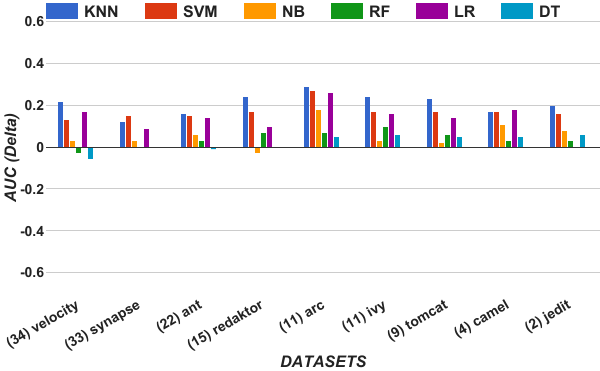
\includegraphics[width=.95\linewidth]{./fig/AUC_untuned.png}
        
  {\bf Figure~\ref{fig:untuned}a:} AUC (pf, recall)
        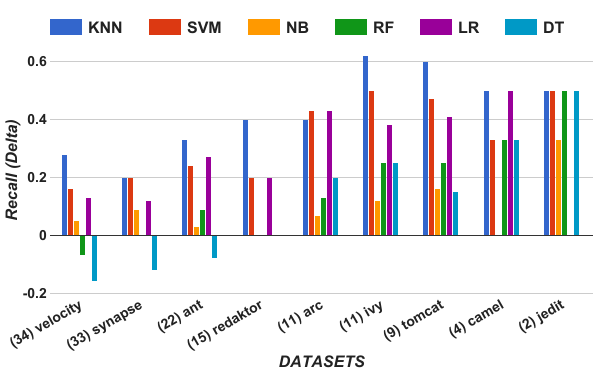
\includegraphics[width=.95\linewidth]{./fig/Recall_untuned.png}
  {\bf Figure~\ref{fig:untuned}c:} Recall
    \end{minipage}%
\begin{minipage}{.5\linewidth}
        \centering
        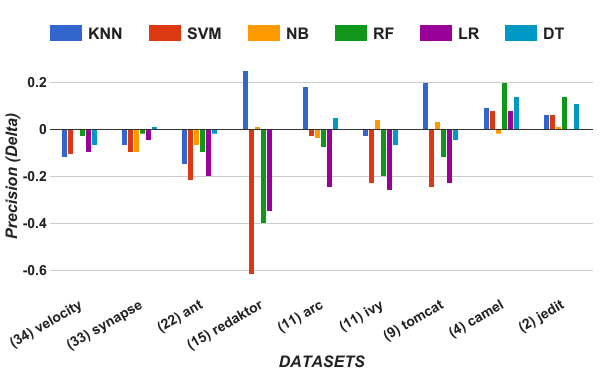
\includegraphics[width=.95\linewidth]{./fig/prec_untuned.png}
  {\bf Figure~\ref{fig:untuned}b:} Precision
        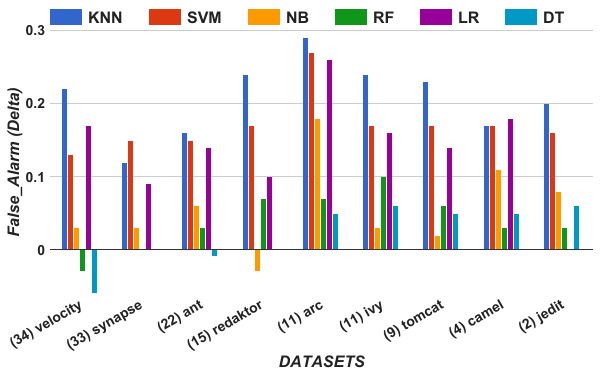
\includegraphics[width=.95\linewidth]{./fig/pf_untuned.png}
  {\bf Figure~\ref{fig:untuned}d:} False Alarm
    \end{minipage}%
    \caption{SMOTE1 improvement over No SMOTE. Legends represent the classifiers mentioned in \tion{classes}}
    \label{fig:untuned}
\end{figure*}

\begin{figure*}[!t]
\begin{minipage}{.5\linewidth}
\centering
        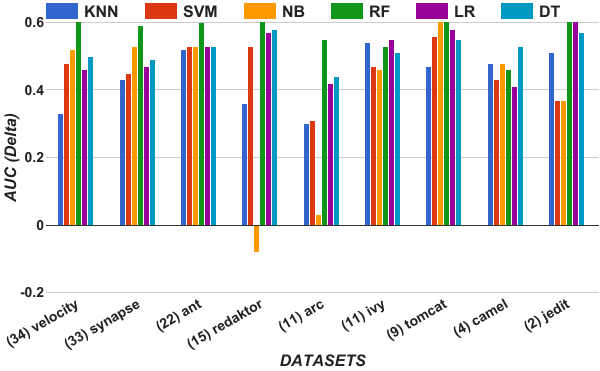
\includegraphics[width=.95\linewidth]{./fig/AUC_tuned.png}
        
  {\bf Figure~\ref{fig:tuned}a:} AUC (pf, recall)
        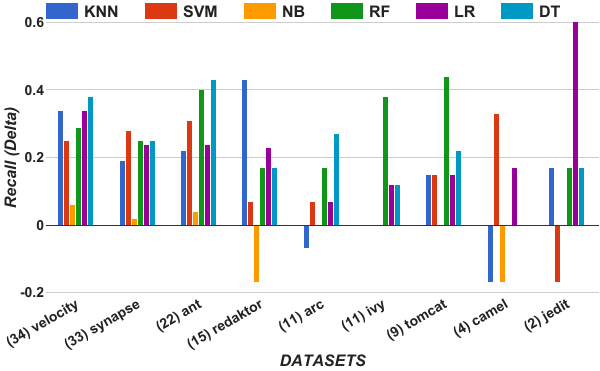
\includegraphics[width=.95\linewidth]{./fig/Recall_tuned.png}
  {\bf Figure~\ref{fig:tuned}c:} Recall
    \end{minipage}%
\begin{minipage}{.5\linewidth}
        \centering
        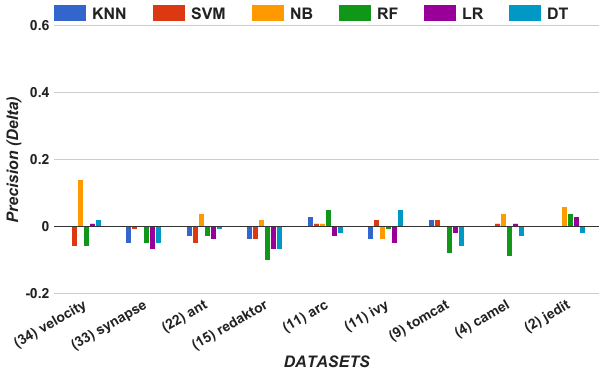
\includegraphics[width=.95\linewidth]{./fig/prec_tuned.png}
  {\bf Figure~\ref{fig:tuned}b:} Precision
        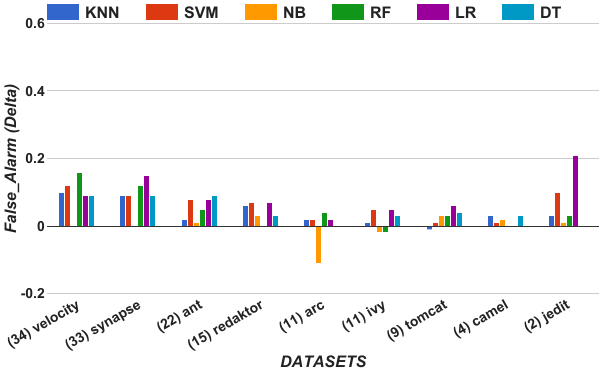
\includegraphics[width=.95\linewidth]{./fig/pf_tuned.png}
  {\bf Figure~\ref{fig:tuned}d:} False Alarm
    \end{minipage}%
    \caption{SMOTE2 improvement over SMOTE1. Legends represent the classifiers mentioned in \tion{classes}.}
    \label{fig:tuned}
\end{figure*}

\section{Results}
\label{sect:results}

\subsection{\textbf{RQ1: Is standard ``off-the-shelf'' SMOTE1 preprocessing method important for defect prediction?}}
Figure~\ref{fig:untuned} represents the improvement of SMOTE1 (median value) against the No SMOTE (median value) results and Figure~\ref{fig:tuned} represents the improvement of SMOTE2 (median value) against SMOTE1 (median value) results. Each figure contains subfigures for all our 4 evaluation measures (mentioned in \tion{measure}) compared with 6 learners (mentioned in \tion{classes}). 



For subfigures (AUC, Recall and Precision) in each Figure~\ref{fig:untuned} and \ref{fig:tuned}:
\bi
\item 
{\em Larger} y-values
are {\em better} 
\item
If the y-value goes {\em negative}, then the corresponding learner performs {\em worse}. 
\ei
For the false alarms, the
plots must be interpreted differently:
\bi
\item
{\em Larger} y-values are {\em worse};
\item
If the y-value goes {\em positive} then
the corresponding leaner
performs {\em worse}.
\ei
Note that, using SMOTE1 on KNN, SVM,
LR (linear regression) often
leads to much larger false alarm increases.
On the other hand,   NB
and RF have much smaller
increase in false alarm.

In these figures, the
X-axis shows all 9 data sets in the decreasing percentage of defective classes from left to right. The corresponding percentage of minority class (in this case, defective class) is written beside each data set. Note that:
\bi
\item
According to the proponents
of SMOTE, SMOTE's improvements should
{\em increase} as we move left to right
across those plots.
\item
No such trend exists in our results for
AUC, precision or false alarms.
\item
For recall, looking left-to-right across
Figure~\ref{fig:untuned}c, we can see
large positive increases on the
right-hand-side than the left.
\ei
% Based on these results,  we can best recommend SMOTE1 when:
% \bi
% \item Trying to improve recall
% for imbalanaced data sets;
% \item
% Using NB or Random Forests.
% \ei

% For SMOTE2 improvement over SMOTE1 (figure~\ref{fig:tuned}), AUC values are shown in subfigure~\ref{fig:tuned}a. Redaktor data set is selected from X-axis, and yellow bar represents NB which corresponds to about $-0.08$ AUC value. This denotes that NB performed worse by tuning the parameters of SMOTE1. The original parameter settings of SMOTE1 worked the best. On the other hand for the same data set, KNN (which is represented in dark blue bar) shows the AUC value of $0.35$. This shows KNN outperformed the ``off-the-shelf'' SMOTE1 when tuned using DE.



% By looking at the results of AUC from figure~\ref{fig:untuned}a, only 4 bars are negative, and rest all the remaining 50 bars (in total 9 data sets with 6 learners in each) have  positive effect by using SMOTE1 as a preprocessing method. We are seeing a maximum improvement of about 30\%. These improvements are quite modest as to ignore the importance of SMOTE.

% Results for precision (in figure~\ref{fig:untuned}b), are not much interesting, but the decrease in precision value is not that arduous except for the redaktor data set. Though we will not recommend using SMOTE whenever we want higher precision value. Since precision is decreased using SMOTE, it was expected to have increased false alarm \cite{menzies2007problems} and the same is observed from figure~\ref{fig:untuned}d. There is an increase in error among false positives but the increase is very minimal.

% As for recall (figure~\ref{fig:untuned}c), only 4 bars are negative, and rest all the remaining 50 bars (in total 9 data sets with 6 learners in each) have positive effect by using SMOTE1. We are seeing a maximum improvement of about 60\%. These improvements are quite steep as to ignore the importance of SMOTE at any point for any learner. It is also observed that performance keeps increasing as target class becomes more minor and minor. This is what was expected after applying SMOTE to imbalance data sets.

\noindent
Summarizing the above:
\begin{lesson1}
We can recommend SMOTE1 for improving recall, and modest improvements in AUC. But  SMOTE1 adversely effect
precision.
\end{lesson1}

\subsection{\textbf{RQ2: Can tuning SMOTE1 achieve better results?}}

Figure~\ref{fig:tuned} shows the results
after applying SMOTE2. All these
plots show the {\em delta} between
the SMOTE1 results and those of SMOTE2.
As before, {\em positive}  values
are better for AUC, recall and precision
wile {\em negative} values are better for false alarms.

The benefit of SMOTE2's tunings are clearly evident in the AUC results of  Figure~\ref{fig:tuned}a:
all learners show large performance improvements. 
Better yet,  as
shown in
Figure~\ref{fig:tuned}b, and Figure~\ref{fig:tuned}d, SMOTE2 does
not adversely effect false alarm and precision.

SMOTE2's benefits for recall are not very
strong (and seem to be strongest for the more balanced data sets on the left-hand-side of Figure~\ref{fig:tuned}c)
but are rarely negative.




% results are dramat
% Now when we look at the results of AUC from figure~\ref{fig:tuned}a, only 1 bar is negative, and rest all the remaining 53 bars (in total 9 data sets with 6 learners in each) have  positive effect after when we tune the parameters of SMOTE1. We are seeing a maximum improvement of about 70\% and on an average 50\% for each learner in all data sets. These improvements are quite steep in nature and just to remind you that these results are improvement over SMOTE1. If we combine the results, then we can surely say to tune the parameters of SMOTE1 and train using any learner, we will get atleast 100\% improvement in most cases.

% We are seeing the similar trend of results for precision (in figure~\ref{fig:tuned}b), just like in Figure~\ref{fig:untuned}b, that even after tuning for precision, we are not seeing much improvement. Though we definitely improved precision slightly than SMOTE1 but the increment is not that large to recommend SMOTE2 or SMOTE1. And even after trying to minimise the false alarm (figure~\ref{fig:tuned}d) value, DE could not find a good parameter setting.

% As for recall (figure~\ref{fig:untuned}c), only 5 bars are negative, and rest all the remaining 49 bars (in total 9 data sets with 6 learners in each) have either positive effect or no effect after tuning. We are seeing a maximum improvement of about 65\% but the average improvement is close to 15\% for each classifiers in all data sets. But these improvements combined with SMOTE1 suggest that we should always tune SMOTE1 whenever the goal is to achieve higher recall.
In summary:

\begin{lesson1}
    For defect data, SMOTE2  
 offers   some  improvements over SMOTE1 for recall
 and dramatic improvements for AUC (pf, recall) without damaging precision or false
 alarm.
\end{lesson1}

Overall, in  Figure~\ref{fig:tuned},
there are very few negative results
(except in precision, where the negatives
are very small). That is, there
seems little to be lost using SMOTE2
but much to gain (e.g. the large AUC improvements).
Based on these results, we strongly
recommend SMOTE2 for handling unbalanced
data sets.

\begin{figure*}[!t]
    \centering
    \begin{minipage}{.33\textwidth}
        \captionsetup{justification=centering,singlelinecheck=off}
        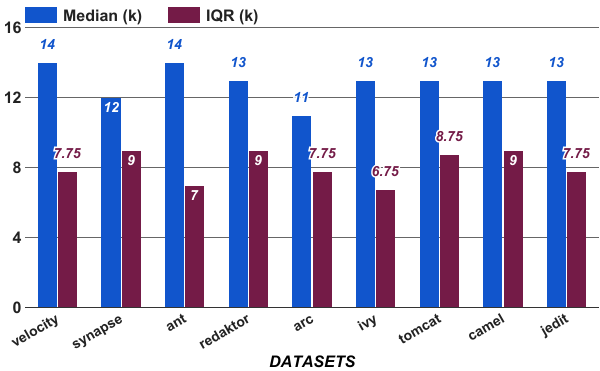
\includegraphics[width=.95\linewidth]{./fig/k.png}
        \caption{Data sets vs Parameter ($k$) variation}
        \label{RQ3:k}
    \end{minipage}%
    \begin{minipage}{.33\textwidth}
        \captionsetup{labelsep=space,justification=centering,singlelinecheck=off}
        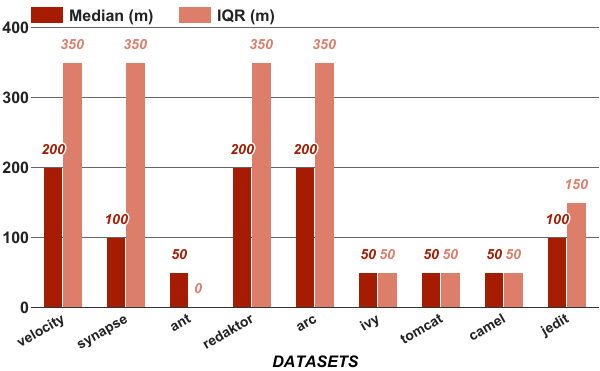
\includegraphics[width=.95\linewidth]{./fig/m.png}
        \caption{Data sets vs Parameter ($m$) variation}
        \label{RQ3:a}
    \end{minipage}
    \begin{minipage}{.33\textwidth}
        \captionsetup{labelsep=space,justification=centering,singlelinecheck=off}
        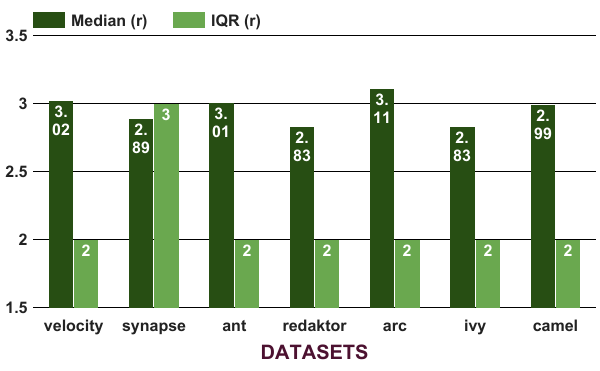
\includegraphics[width=.95\linewidth]{./fig/r.png}
        \caption{Data sets vs Parameter ($r$) variation}
        \label{RQ3:b}
    \end{minipage}
\end{figure*}

\subsection{\textbf{RQ3: Do different data sets
      need different configurations with SMOTE2?}}

Figures \ref{RQ3:k}, \ref{RQ3:a}, and \ref{RQ3:b} show the results of tuning for each data set when recall is considered as evaluation goal. These parameter settings are found by each learner for that data set.
On display in each set of vertical bars are
the median values generated across 15 evaluations.
Also, shown are
the inter-quartile range (IQR) of those tunings (the IQR is the 75th-25th percentile values and is a non-parametric measure of variation
around the median value). Note that in Figure \ref{RQ3:a}, IQR=0 for  ant data set where tuning
          always converged on the same final value.

  These figures
show how tuning selects the different ranges  of
parameters.
Some of the above numbers are far from the standard values; e.g. Chawla et al.~\cite{chawla2002smote} recommend using $k=5$ neighbors yet in our data sets, best results were seen using $k \approx 13$. On other hand it was suggested to use $m=900$ by ~\cite{pears2014synthetic}.
Clearly,
best results from tuning
vary with each data set.

Clearly:
\begin{lesson1}
    DE finds different ``best'' parameter settings for SMOTE2 for different data sets.
\end{lesson1}
 That is,  reusing tunings  suggested  by  any other  previous study  for any data set is \underline{{\em not}} recommended. Instead,  it is better to
      use  automatic  tuning  methods  to find the best tuning parameters for the current data set.
      

\begin{figure}[!t]
  \captionsetup{justification=centering}
  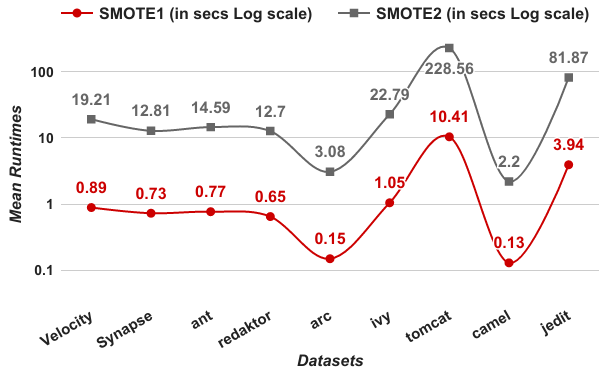
\includegraphics[width=\linewidth]{./fig/runtimes.png}
  \caption{Data sets vs Runtimes}
  \label{runtime}
\end{figure} 

\subsection{\textbf{RQ4: Is tuning impractically slow?}}

Search-based SE methods can be very slow. Wang et al.~\cite{wang2013searching} once needed 15
years of CPU time to find and verify the tunings required for software
clone detectors. Sayyad et al.~\cite{sayyad2013scalable} routinely used
$10^6$ evaluations (or more) of their models in order to extract
products from highly constrained product
lines. Hence, before recommending any
search-based method, it is wise to consider the runtime cost of that
recommendation.

To understand our timing results, recall that SMOTE2 uses
Algorithm~1. Based on the psuedocode
shown above, our pre-experimental expectation is that
tuning will be three to fives times slower than not tuning.  
Figure~\ref{runtime} checks if that theoretical
holds true in practice. Shown in circle and square markers are the
  runtimes required to run SMOTE1 and SMOTE2 respectively.  The
  longer runtimes (in square) include the times required for DE to find
  the tunings. Overall, tuning slows down the training by a factor of up to
  five (which is very close to our theoretical prediction).

\begin{lesson1}
    Tuning with DE makes training four to five times slower, but the improvements which we get for AUC and recall is quite advantageous.
\end{lesson1}




\section{Threats to Validity}
\label{sect:validity}

As with any empirical study, biases can affect the final
results. Therefore, any conclusions made from this work must be considered with the following issues in mind:

\textbf{\textit{Sampling bias}} threatens any classification experiment; i.e., what matters there may not be true here. For example, the data sets used here comes from the PROMISE~\cite{promiserepo} repository and were supplied by one individual. Also even though we used 7 open-source data sets for Software Defect prediction (Table~\ref{tb:dataset}) which are mostly from Apache, and some are proprietary projects, there could be other datasets for which our results could be wrong.

\textbf{\textit{Learner bias}}: For building the defect predictors in this
study, we selected each learner with default parameters like k=8 to use in k-Nearest Neighbor. Since there are studies previously talking of using some predefined parameters based on their conclusions. Classification is a large and active field and any single study can only use a small subset of the known classification algorithms.

\textbf{\textit{Evaluation bias}}: This paper uses 4 measures of evaluation but there are other measures used in software engineering which includes Accuracy, Fscore. Measuring performance with more measures is left for future work.

\textbf{\textit{Order bias}}: With each dataset how data samples are distributed in training and testing set is completely random. Though there could be times when all good samples are binned into training and testing set. To mitigate this order bias, we run
the experiment 25 times by randomly changing the order of the data samples each time.

\section{Conclusion}
\label{sect:conclusion}

We were able to reproduce the baseline paper "Revisiting the impact of classification techniques on the performance of defect prediction models" with the same conclusions what Ghotra et al. found. But for class imabalance problem, it is concluded to get better AUC and recall, SMOTE needs to be performed. The improvements in AUC and recall with tuning SMOTE is dramatic. Tuning is important if we have a specific tuning goal like maximizing AUC or recall. When comparing the run times against SMOTE~1, SMOTE~2 is about three to five times slower.

\section{Future Work}
\label{sect:future}
In future, we plan to work on other similar issues like:
\bi
 \item Tuning SMOTE and learners at the same time and comparing against the results of No SMOTE, SMOTE~1, and SMOTE~2.
 \item Predicting the quantities of defects which is regression based model rather having a binary based classification model with tuning.
\ei

\balance

\bibliographystyle{ACM-Reference-Format}
\medskip
\bibliography{main}

\end{document}


\end{document}

